% !TEX root = ./thesis.tex
\chapter{Integrating Land Use Change Modelling with Connectivity Modelling, a Case Study in Montérégie, Southern Québec}
\begin{center}
{Valentin Lucet$^{1}$, Andrew Gonzalez$^{1}$}\\
\end{center}
\textit{Author Affiliations:}\\
\normalsize{$^{1}$Department of Biology, McGill University}\\

\newrefsection

\section{Abstract}

Ecological connectivity, defined as the extent to which the landscape supports the movements of organisms, can be strongly affected by land use. It is an important component of the resilience of populations in heterogeneous and fragmented landscapes. Land use changes such as urban sprawl and agricultural intensification intensify habitat fragmentation and landscape homogenization, leading to the erosion of ecological connectivity. The Montérégie region in southern Québec, where this work takes place, is experiencing urban growth and sprawl. We present a framework that integrates land-use, climate change and connectivity modeling to forecast future changes in connectivity, using a combination of statistical modeling, MCMC-based simulations, and circuit theory. We used a hybrid modeling approach to project future land use changes using different climate scenarios, and estimate future changes in functional connectivity flow for 5 different umbrella species. We explore the flexibility of a scenario approach in forecasting the range of possible futures for ecological connectivity in the region and derive potential insights for the hypothetical design of a local network of connected protected areas resilient to future landscape change. In conclusion, we highlight the need for a multi stakeholder approach in the definition of scenarios and conservation priorities.\\

\newpage

\section{Introduction}
\vspace{2em}

%[intro paragraph]
The goal of connectivity conservation planning is to preserve the continuity of habitat in a landscape, by identifying and protecting habitat patches and corridors necessary to maintain the movement of plants and animals \citep{keeley_thirty_2019}. Ecological connectivity, defined as the extent to which the landscape facilitates or impedes the movement of organisms \citep{crooks_landscape_2006}, is a critical component of the resilience of populations in heterogeneous and fragmented landscapes \citep{gonzalez_spatial_2017}. Connectivity conservation planning methods do not typically account for risks associated with future land use and climate change, two main drivers of the erosion of ecological connectivity. Here, we ask whether those methods can be improved by taking into account those risks. To do so, we integrate a connectivity model with a land use change model including climate scenarios.

% [CC as an adaptation measure, but CC designs are vulnerable]
Connectivity conservation has often been identified as a method for adaptation to climate and land use change \citep{costanza_landscape_2019}. One recurring argument is that preserving landscape connectivity could be critical for ensuring that species can shift their ranges \citep{krosby_ecological_2010, keeley_making_2018} in response to climate change. Another argument is that it is more important than ever to connect habitats in landscapes increasingly hostile to species movement \citep{ellis_anthropogenic_2010}. These arguments make the case for the design of Connected Protected Area Networks (CPAN, \cite{opdam_ecological_2006, stewart_corridors_2019, gonzalez_spatial_2017}). Those networks are meant to allow the movement of species across multiple scales, which may require them to include both natural and semi-natural habitat, with different levels of protections \citep{daloia_coupled_2019}. This heterogeneity is likely to be reinforced by the multiplicity of urban and land use planning practices that exist on the landscape, making CPAN designs particularly vulnerable to changes in land use. It is therefore important to test which specific CPAN designs would be most resilient to future  change.  One possible approach to exploring this resilience is to use landscape-level models that project the future state of land-cover.

%[Land use change and climate models often  used in conservation]
Land use change models have often been used in conservation planning (for example, see \cite{echeverria_spatially_2008} or \cite{lesschen_identification_2007}). They allow researchers to test the efficiency of a given conservation plan in the face of expected land use change. Similarly, climate models are often used in conservation, for example to assess whether protected areas will include future species ranges that are shifting due to climate change \citep{araujo_would_2004, heller_targeting_2015}. They are also central in species distribution models \citep{porfirio_improving_2014}, a classic tool in conservation research. Both types of models are increasingly common in research focused on landscape planning for ecological connectivity.

% [what about those models in CC context?]
Connectivity researchers have studied how past changes in land use can explain current connectivity patterns \citep{dupras_urban_2015, henareh_khalyani_spatial_2013, vergara_deforestation_2013, patru-stupariu_using_2013} and multiple connectivity measures have been developed, one specifically in this context \citep{saura_new_2007}. But beyond these historical analyses, land use models are becoming more common \citep{correa_ayram_habitat_2015}. For example, \cite{rubio_sustaining_2012} identified a network of forest patches resilient to land use change under multiple scenarios in Spain. Similarly, \cite{piquer-rodriguez_future_2012} integrated land use change and connectivity models to identify under-protected areas by projecting land use change trends. \cite{huang_simulating_2018} also used land use change models to assess potential impacts on functional connectivity in China. \cite{albert_applying_2017} used a land use change model to forecast changes in species networks. From these examples, we can see that combining land use change modelling and connectivity modelling does not yet have a fully established methodology. In its emerging form, it simply consists of running a land use change model on a given landscape, and comparing changes in the connectivity measure of choice between time steps \citep{perkl_urban_2018}.

% [back to what we want to do]
Climate change can interact with land use change in ways that impact biodiversity \citep{oliver_interactions_2014} It is therefore likely that connectivity models integrating these two drivers would improve connectivity conservation methods such as CPAN design. Yet, in a recent review, \cite{costanza_landscape_2019} have found that connectivity methodological frameworks rarely combine  land use change and climate change. Here, we build on recent connectivity modelling work using circuit theory, by pairing it with a hybrid land use and climate change model \citep{albert_applying_2017}. The model we develop uses a combination of statistical modelling and simulations based on a Markov Chain Monte Carlo (MCMC) method, combining Random forests (RF) models with a Cellular automaton (CA) model. We use this RF-CA model to project future land use changes and estimate the changes in potential functional connectivity for five different umbrella species, under different climate change scenarios. We also derive potential insights for the design of a hypothetical regional network of connected protected areas resilient to future landscape change. In addition, we provide an analysis of past land use change trends in our study region, the Montérégie region in southern Québec.

%[we are building on past work]
This work is the continuation of recent research efforts on the connectivity of the region: \cite{albert_applying_2017} and \citep{rayfield_priorisation_2018}. In a seminal paper, \cite{albert_applying_2017} laid out some of the methodological steps we follow such as umbrella species selection and habitat suitability analysis. They also included a simple land use change model that was parameterized to replicate plausible change in the region. \cite{meurant_selecting_2018} developed the criteria for reducing the number of focal species from fourteen to five. They showed that because species had redundant connectivity needs, modelling the needs for 5 species resulted in qualitatively similar results than when modelling the needs of all 14 species, such as in Albert et al. (\citeyear{albert_applying_2017}). While Rayfield et al. (\citeyear{rayfield_priorisation_2018}) extended the spatial scale of the analysis to include the Saint Lawrence lowlands ecoregion, they demonstrated that we could exploit this redundancy to reduce the computing time needed for the connectivity analysis. This is an important development because land use change simulations are also computationally intensive.

% \subsubsection*{\textit{Modelling potential functional connectivity}}
%[description of connectivity]
Connectivity is a dynamic property of the landscape: it changes across time and space \citep{beyer_functional_2013}. It is also scale and species specific, varying according to the needs of each species and because those needs also vary depending on the time of the year, life history, and on the species’ habitat range and preference \citep{anderson_scale-dependent_2005}. It is important to distinguish structural connectivity from functional connectivity \citep{kindlmann_connectivity_2008}. While structural connectivity strictly refers to how animal movement is mediated by the configuration of habitat features in the landscape, functional connectivity is based on species’ preferences for such features and how they move among them. Functional connectivity modelling therefore attempts to model the extent to which the landscape meets the need of a specific species or set of species.

%[functional versus PFC]
There has been a trend in the recent literature to focus on functional connectivity, as it is regarded as a more realistic representation of  the landscape’s capacity to facilitate species movement than structural connectivity. However, functional connectivity analyses require direct animal movement data or genetic data for model fitting and for validation (for example, see \cite{beyer_functional_2013, milanesi_three-dimensional_2017}). This type of data is costly to acquire, especially when needed for many species. For this reason, much of current functional connectivity modelling, including the methods of this chapter are in fact modelling “potential functional connectivity”, or PFC. PFC models do not necessarily rely on actual movement data, but are based on other kinds of knowledge of species habitat preferences and movement behaviors, for instance, from expert knowledge and literature reviews. This makes PFC well suited to the task of this paper.

%[we combine the PFC and redundancy concepts]
Here we model  PFC for the 5 focal species identified by  \cite{meurant_selecting_2018} and use the workflow of \citep{rayfield_priorisation_2018} for habitat suitability and connectivity analysis. We complement this framework with the RF-CA land use model. It is important to note that the primary goal of this chapter is not to explain the drivers of land use change in the region, but to provide a sufficiently realistic simulation to replicate the trends in land use change that have been observed historically, and to project those trends forward into the future.  \\

\section{Methods}

Our workflow is divided into two major steps: land use change modeling and connectivity modeling. Two workflow figures describe the steps and methods involved (figure \ref{fig:workflow1} and \ref{fig:workflow2}). \\

\subsubsection*{\textit{Software tools and reproducibility}}

All work was conducted in the R statistical software version 3.6.2 "Dark and Stormy Night" \citep[see][]{R}). The data and code for this thesis are available at \href{https://github.com/VLucet/landchange-connectivity-monteregie}{this GitHub repository}.

We used ST-Sim version 2.2.10, scripted in R with the help of the rsyncrosim package version 1.2.0. ST-Sim ran on Linux (Ubuntu 18.04) via Mono 6.4. Many steps of data preparation were conducted in GRASS GIS 7.8.

A note should be added on data availability and reproducibility. A few datasets were not obtained from open sources. These datasets are marked in red in figure \ref{fig:workflow1}. The Canadian census data was obtained through the University of Toronto's CHASS (Computing in the Humanities and Social Sciences) Data Centre, which requires institutional access. This makes the Random Forest analysis not reproducible. In addition, data on protected areas in Montérégie was obtained  via the RMN (Réseaux des milieux naturels protégés du Québec) under a limited license, which makes the Land use change modeling via ST-Sim not fully reproducible. However, the final results of those steps are made open (under the form of csv files), and therefore the generation of the main figures are reproducible via the use of various software (i.e. docker, renv, and more). \\

\subsection{Land use change modelling}
Land use change modelling is a prolific subfield of land systems science which has spurred a broad diversity of approaches \citep{dang_review_2016, noszczyk_review_2018}. Beyond the many methods published, there is a large number of applications and software tools available for research - although their openness and accessibility varies \citep{moulds_open_2015}. Papers that compare frameworks and results across tools and methods are rare \citep{pontius_comparing_2008, pontius_comparison_2005, sun_comparison_2018}. Although a full review of land use change modelling methods is beyond the scope of this chapter and this thesis, we will introduce the key concepts.

Land use change models can be classified according to their level of focus on land use change drivers, from phenomenological (“top down”) to more mechanistic approaches (“bottom up”). Given the simplicity and ease of use of phenomenological models, and the extra demands of mechanistic models, most approaches to land use change modelling fall between these two extremes, and a certain number of “hybrid” approaches have been developed \citep{sun_comparison_2018, jokar_arsanjani_integration_2013}. The approach we take in this chapter is not strictly phenomenological and introduces some mechanistic understanding of land use change, and can therefore be qualified as a hybrid method.

Our land use change model is set up in two steps: a land use suitability analysis and an allocation algorithm. In a nutshell, the suitability analysis step determines how likely each pixel is to acquire a given state by producing a probability surface, predicted based on spatial data, and the allocation step simulates change over that surface. The allocation is a Markov process informed by the results of the first step. This Markov process is embellished to include conditions such as neighboring rules and transition size distributions.

The two steps framework we just outlined allows us to combine the power of markov chains with the flexibility of statistics. Any method can in theory be used to determine the probability surface (although linear and logistic regression techniques are most common), and complex algorithms can be written to determine rules of allocation. The simplicity and flexibility of this framework explains the popularity of common land use change modelling frameworks like CLUE  (Conversion of Land Use and its Effects \cite{verburg_modeling_2002, verburg_combining_2009}). \\

\subsubsection{The RF-CA modelling framework}

Our choice of statistical framework was done considering at least three factors: computing time, prediction power and capacity to deal with spatial processes. Computing time is an important factor because fitting models to large datasets can be time consuming. Capacity for dealing with spatial processes varies across methods. Finally, statistical frameworks sit along a continuum that emphasises more or less inference and prediction. A Bayesian model will be more easily thought of as a tool for statistical inference, whereas a neural network will be used more with predictive power in mind.

We chose Random Forests (RF) as a statistical framework. RFs are a tree-based machine learning algorithm that generates a “forest” of randomized decision trees, which have the property to be independent to each other and identically distributed. RFs can be easily “grown’ in parallel, which reduces computation time. RFs possess a strong predictive power, but can still provide metrics of variable importance, providing an interesting balance between inference and predictive power.

For the allocation step, we use an advanced cellular automata (CA) modelling tool (markov-chain based) called ST-Sim, a package of the free software SyncroSim. ST-Sim allows for more complex simulation than a classic CA as it allows for complex neighbouring rules with state and age cell tracking. It is also built to handle large datasets and can be scripted to run in parallel. It is important to note that although it is the first time RF is used with ST-Sim (to our knowledge), this hybrid modelling approach (coined “RF-CA”) has been used successfully in other land use change modelling projects \citep{kamusoko_simulating_2015, gounaridis_random_2019}. ST-Sim can be customized to function under multiple different types of inputs. The two main inputs are transition probability and transition targets. Readers should refer to Daniel el al. (\citeyear{daniel_state-and-transition_2016}) for a more in-depth overview of how ST-Sim and SyncroSim functions. \\

\subsubsection{Data sources and preparation}

\subsubsection*{\textit{Land use change data}}

For most modelling frameworks, the raw source of land use change data is remote sensing data. Because producing land use change data from remotely sensed imagery was beyond the scope of this thesis, we looked for a curated dataset. Agriculture and Agri-Food Canada (AAFC) produces a dataset of land use in Canada at a 10 years interval and at the resolution of 30 meters (the resolution is the dimension of a pixel in a spatial grid, or raster data, and is an important property of land use datasets). This dataset provides land use data for the years of 1990, 2000, 2010. We found this data product, referred to hereafter as the AAFC data  to be the right fit for our approach: the data production method of the AAFC  data is consistent, meaning that similar methods have been used to produce all three maps at different time points. Consistency in data production methods is key as it makes the computation of change between time points more reliable.

This data is not without limitations: compared to other data products - such as the Québec Ministry of the Environment land use dataset or the Statistique Québec land accounting dataset - the AAFC dataset is not very detailed: only a few land use categories are identified, and important information for suitability analysis such as forest age and forest density are missing.

Another limitation is the coordinate reference system (CRS) in which this dataset is available: it is projected in a UTM projection system, which is not the standard CRS used by other data products that usually covers Québec and emanates from open data portals in the province. This makes direct comparison (pixel by pixel) to those others datasets difficult. Finally, the AAFC data does not differentiate between road types, which lead us to source road data from the Adresses Quebec dataset.\\

\subsubsection*{\textit{Forest types and dynamics under climate change}}

The AAFC data does not differentiate between different forest types. However, our connectivity analysis relies on an analysis of habitat suitability, which is reliant on knowing the preferences of different species for different forest types (see section of habitat suitability analysis for more details). In order to integrate dynamics of forest types into our simulations, we relied on the results of a separate set of simulations that were run in LANDIS, a free and open source software designed to model forest growth. Those simulations were run by Boulanger and Larocque (unpublished, see Appendix 3) for the extent of the Saint-Lawrence lowlands ecoregion, in the context of a research contract with the MELCC (Ministère de l'Environnement et de la Lutte contre les changements climatiques). The LANDIS simulations do not include land use change and therefore can not be directly merged into our simulations. Instead, we parameterized the changes in forest types from the results of the LANDIS simulations. A more detailed methodological description of the LANDIS simulations is to be found in the Appendix 3.

We source two different sets of "parameters" from these simulations: first, forest type data in 2010 was used as a starting point for the forecast scenarios. Second, a set of transition multipliers were extracted from the simulations and was used to reflect different forest dynamics under different climate change scenarios. These are described in more details in the "Model Execution" section.\\

\subsubsection*{\textit{Explanatory variables}}

A diversity of drivers of land-use change can be found in the literature. Some general group of variables can be identified: an important distinction can be made between physical and social-economical variables. Proxy variables for land use change drivers used in this chapter were selected among commonly recognized predictors of land use change.

A digital elevation model was used to derive elevation data (continuous variable). We used the data product “SRTM 30m” available throughout the Google Earth Engine data portal to generate this variable. This data was already available at a 30 m resolution.

We used the Canadian Census for the years of 1991, 2001 and 2011, provided by Statistics Canada, to extract two variables: population change (1991 -2001) and average income. The data was not available in a spatial format and had to be turned into a spatial object in R before being rasterized. The data was collected at the lowest aggregation level available: the denomination area (DAs) or the Enumeration area (EAs) depending on the census year (see table \ref{tab:variables} for the full description of variables and data sources).\\

\subsubsection*{\textit{Data preparation}}

The first step consisted in reclassifying the AAFC land use dataset into 4 categories: the 3 categories of our land use change model plus roads and wetlands. Then we aggregated the rasters by a factor of 3 (using the mode of the neighborhood, changing the resolution to 90m). We applied this aggregation to all rasters (for continuous data we used the mean and not the mode). This allowed us to reduce run time as well as memory requirements. Roads were removed during aggregation: this was necessary as the process tends to break them up, creating holes in them. Major roads from the Adresses Quebec dataset were rasterized and patched on top of the resulting maps. Then, all the pixels classified as forest were reclassified as null, and the resulting maps were patched with the forest cover from the LANDIS simulations' starting conditions (state of forest types in 2010). Some cells remained null as the forest cover in 1990 was larger than that of 2010. We filled those NULL values using modal imputation under two different neighbourhood window sizes (13 and 25 pixels). Next, a 5km buffer was added around Montérégie so as to improve the Circuitscape results later down the pipeline (see the Connectivity Analysis section). Not all NA cells were due to the difference in forest cover between 1990 and 2010, some were due to the fact that the LANDIS run did not cover some parts of the 5km buffer. Those cells were filled with the value corresponding to the forest type Mixed Forest of Medium Age. We decided on this imputed value because it is among the most suitable for all species and therefore unlikely to cause significant changes in the Circuitscape runs, even if it does not correspond to the mode or the mean for the region. In addition, because no change takes place in the buffer, those values can be equivalent to a "padding" around the landscape.

A second step was the preparation of the explanatory variables. Vector data was rasterized when needed. A significant effort was invested in working with the Canadian Census data, as Statistics Canada does not make available a spatial dataset for their census data. Therefore, the geometries of DAs and EAs had to be matched with the corresponding line in the Census dataset, based on the unique EA and DA IDs. Some of these (between 2 and 5 \% of the total number of DAs or EAs, depending of the time steps) have remained unmatched due to discrepancies between the (spatial) boundaries datasets of EAs/DAs available and the EAs/DAs listed in the StatsCan dataset. This led to areas with NAs values. These areas could not be ignored in our random forest model and had to be imputed. We used mean imputation for lack of a better method but are aware of the large number of issues associated with this practice \citep[see][]{lodder_impute_2014}.

Finally, all variables were extracted and turned into tabular data. Only relevant pixels (i.e. rows in the dataset) were kept to model each transition. For instance, only forest and agricultural land pixels were kept to model urbanization. The variables were standardized prior to running the model. We used the \verb|tidymodels| framework (version 0.1.0) in R to pre-process our tabular data and run our random forest models. \\

\subsubsection{Preliminary analysis of past land use change}

To better understand land use patterns in the region, we ran some preliminary analysis on land use change data at the municipality level. Montérégie is made up of 177 different municipalities. We generated land use matrices (amount of each land use category) and land cover transition matrices for the first timestep of our dataset (1990 to 2000) for each municipality and for the land use categories corresponding to our model. We then performed multivariate analyses by running a first ordination using PCA (Principal Component Analysis), and then using Ward clustering \citep{legendre_ordination_2012}.
Because municipalities in Montérégie have variable size, the amount of change in each municipality needs to be standardized. The data was normalized prior to the ordination to reflect relative amounts of change in each municipality. We used the \verb|vegan| package in R to produce such plots.\\

\subsubsection{Model Execution}

\subsubsection*{Random forest}

\subsubsection*{\textit{Calibration \& validation}}

Land use change data has a tendency to be highly unbalanced, because over a certain time period, the amount of pixels that have transitioned into a new state is usually small compared to the amount that did not transition into a new state. In the case of Random forest models, there are a few ways to deal with such imbalance. In this work, we simply down-sampled our dataset to reach a ratio of 2:1 (i.e. 2 pixels that did not transition for each pixel that did transition).

The RF model was calibrated on a training partition (70\% of the down-sampled dataset) for the timestep of 1990 to 2000. The model was then spatially validated on a test partition (30\% of the dataset), and then temporally validated for the timestep of 2000 to 2010 (100\% of the dataset for this timestep). \\

\subsubsection*{\textit{Performance evaluation}}

There are a number of ways to evaluate model performance in the context of land use change predictions. We used three different approaches:
\begin{itemize}
\item We report the goodness of fit ($R^{2}$ between data and prediction) of the random forest model, as well as variable importance (evaluated as gini impurity score).
\item We used a ROC curve with Area Under the Curve (AUC) to compare true observed change with the predicted probabilities of transition. This method is often used in landscape ecology and land use change modeling \citep{pontius_recommendations_2014}.
\item We used a Conventional Cross Validation (CCV) method for the reporting of AUC values, with 10 folds, for which we also produce a measure of AUC with ROC curves.\\
\end{itemize}

\subsubsection*{ST-Sim}

ST-Sim \citep{daniel_state-and-transition_2016}  is a State and Transition model (STM) and can therefore be provided with probabilities of land use change. However in order to integrate the results of our random forest models, we parameterized ST-Sim differently than a classic STM. All probabilities are set to 1, and we leverage the spatial multiplier feature of the software. We provide our fitted probability surfaces (outputs of the RF models) as spatial multipliers. Therefore, each pixel's probability of change is provided by that surface (multiplied by 1). This is not enough to reproduce past trends in land use change: we need to provide transition targets to the allocation algorithm. These targets are directly based on the amount of land change between 1990 and 2010 for time steps 1990 - 2010.\\

\subsubsection*{\textit{Model definition}}

The ST-Sim model uses three states: Forest, Urban and Agriculture. Forest was further subdivided into classes of age and type, derived from the LANDIS outputs: three forest types (\textbf{deciduous}, \textbf{mixt}, and \textbf{coniferous}) and three age classes (\textbf{young}, 0-20 yrs ; \textbf{medium}, 20-40 yrs ; and \textbf{old}, 40+ yrs) for a total of 9 classes.
The model allows for 4 groups of transitions:
\begin{itemize}
\item{\textbf{Urbanisation}}: groups \textbf{deforestation} (Forest $\Rightarrow$ Urban) and \textbf{agricultural loss} (Agriculture $\Rightarrow$ Urban).
\item{\textbf{Agricultural expansion}} (Forest $\Rightarrow$ Agriculture).
\item{\textbf{Forest Internals}}: groups the 72 combinations of forest change between the 9 forest internal states.
\end{itemize}
The model takes in 3 different strata. A stratum in ST-Sim refers to a subset of the entire landscape being considered for analysis. Strata are typically used to divide the overall landscape into regions or zones, each of which can have different model parameters specified. The three stratum are:
\begin{itemize}
\item{Primary stratum:} delineates Montérégie from the  surrounding buffer and highlights protected areas.
\item{Secondary stratum:} delineates municipalities of the region, to allow to set targets specific to each municipality.
\item{Tertiary stratum:} delineates LANDIS land types, to allow to set transition multipliers for forest types that match the LANDIS simulations. \\
\end{itemize}

\subsubsection*{\textit{Spatial dependency}}

Under the parameters defined so far, ST-Sim takes care of transitioning the amount of land corresponding to the targets it is fed, and will do it probabilistically across the landscape according to the probability surface (spatial multipliers). There is an additional way to restrict this change via Adjacency parameters, which are essentially neighborhood rules. Adjacency rules were defined from basic assumptions about transition spread. The list of neighborhood rules given for each transition type (or group) is provided in the appendix table \ref{tab:neigh_rules}.

We added one more constraint for the Forest Internals group: the Time since Transition parameter which sets a minimum time of 20 years (2 timesteps) in between transitions between Forest  types states.\\

\subsubsection*{\textit{Scenario definition}}

In the subsequent description, we make the distinction between:
\begin{itemize}
\item{\textit{historic runs}}, parameterized to reproduce the changes that happened between 1990 and 2010 in the region, with a different set of transition targets for 1990-2000 and 2000-2010.
\item{\textit{forecast runs}}, parameterized to project forward an average of the trends observed in the two decades, with a single set of transition targets (average of the two 1990-2000 and 2000-2010 targets) and for which only certain set of spatial multipliers change depending on climatic scenarios.
\end{itemize}
We defined two land use change scenarios, crossed with two different climate change scenarios, plus a control climate scenario. Those six scenarios in total are designed to  encompass the realm of possible future habitat changes for our 5 focal species.
The two land use change scenarios are:
\begin{itemize}
\item{\textbf{Business As Usual (BAU)}}: the land use change trends are projected forward into the future with no alteration to those trends.
\item {\textbf{Business As Usual + Reforestation (R)}}: the land use change trends are projected forward into the future, and reforestation is randomly occurring, converting to forest as much land as is lost through urbanization, for every timestep.
\end{itemize}
The climate scenarios influence the probability of transitions between forest types (i.e. succession and disturbances) they subsequently influence habitat suitability and connectivity. The three climate scenarios are:
\begin{itemize}
\item{\textbf{Historic (Hist)}}: No forest change: forest remains as it was in 2010. This is equivalent to a control treatment.
\item{\textbf{Baseline (Base)}}: Forest change continues as it does in today's climate.
\item{\textbf{RCP 8.5 (RCP8)}}: The forest changes according to the emissions scenario RCP 8.5, characterized by increasing green-house gas emissions, high rates of population growth, modest GDP growth and low rates of technological development and uptake. It is the most severe of the future scenarios \citep{ipcc_summary_2013}.\\
\end{itemize}

\subsubsection*{\textit{Details of scenario parameters}}

We ran a total of seven scenarios (one historic run and six forecast runs). Two behaviors remain constant in all seven scenarios: no land use change  takes place in the 5km buffer. In addition, new forest laid by the reforestation transition does not change state for the remainder of the simulation (this is because LANDIS does not provide land type data for new pixels). Therefore, reforestation always produces a forest of the class "Medium Deciduous". In all scenarios described, ST-Sim with decadal time steps, for 10 iterations (10 MCMC realization).

The final list of scenarios is the following:
\begin{itemize}
\item Historic run - 1990 to 2010 \textbf{(Hist)}. In this historic run, the forest type for all three time steps was taken from the LANDIS inputs (forest type data 2010). This is of course not accurate, but because no change is allowed to take place, this is not a problem and it is only there to allow consistency and comparison with the other scenarios.
\item Forecast land use BAU - Historic climate - 2010 to 2100 \textbf{(BAU-Hist)}
\item Forecast land use BAU - Baseline climate - 2010 to 2100 \textbf{(BAU-Base)}
\item Forecast land use BAU - RCP 8.5 climate - 2010 to 2100 \textbf{(BAU-RCP8)}
\item Forecast land use reforestation - Historic climate - 2010 to 2100 \textbf{(R-Hist)}
\item Forecast land use reforestation - Baseline climate - 2010 to 2100 \textbf{(R-Base)}
\item Forecast land use reforestation - RCP 8.5 climate - 2010 to 2100 \textbf{(R-RCP8)}\\
\end{itemize}

\subsection{Habitat suitability and connectivity modelling}

Connectivity modeling is similar to land use change modeling inasmuch as the diversity of methods at the researcher’s disposal is large \citep{calabrese_comparison_2004}. As mentioned in the intro, we implemented an analysis of Potential Functional Connectivity, or PFC. A typical PFC modeling workflow can be broken down to 3 steps: species selection, Habitat suitability modeling and connectivity analysis. The three steps are described below, and the methodology partially follows the methodology of Rayfield et al. This part of the methods is summarized in figure \ref{fig:workflow2}.\\

\subsubsection{Species selection}

Species selection is unchanged from Rayfield et al. The five species chosen are presented in the appendix table \ref{tab:species}. It was demonstrated that modeling the connectivity needs of those 5 species was equivalent to modeling the needs of 14 species in the study region \citep{meurant_selecting_2018, albert_applying_2017}\\

\subsubsection{Habitat suitability}

Habitat suitability analysis consists in reclassifying land use data into a resistance surface which is then used to model connectivity. For each of the maps obtained from the land use change analysis (for each of the timestep in every iteration and for each of the 5 species), we followed the following steps to reclass land use into resistance:
\begin{enumerate}
\item Classify the landscape as \textbf{forest} and \textbf{non forest}.
\item Reclassify non-forest pixels into resistance following the supplementary tables in  \citeauthor{rayfield_priorisation_2018}, with only a few alterations. See table \ref{tab:key_non_forest} for the reclassification key.
\item Clump the forest landscape into contiguous \textbf{patches} using queen case neighborhood (includes diagonal).
\item Reclassify pixels in all patches as suitable (value = 1) unsuitable (value = 0) or moderately suitable (value = 0.5), based on forest age and type, and following guidelines in the supplementary tables in  \citeauthor{rayfield_priorisation_2018}.  The key for such reclassification is recorded in table \ref{tab:suit_pixls}.
\item  Compute the mean patch value based on the clumped outputs.
\item Classify each patch as \textbf{possibly suitable} or \textbf{unsuitable}, with a cut-off value of 0.5.
\item Among the suitable patches, calculate their size.
\item Classify \textbf{possibly suitable} patches into \textbf{fully suitable} patches or \textbf{too small} patches based on their size, using the values provided by \citeauthor{rayfield_priorisation_2018} (see table \ref{tab:patch_size}).
\item Reclassify patches into resistance, once again following the guidelines in \citeauthor{rayfield_priorisation_2018}'s supplementary tables. See table \ref{tab:hab_or_not} for the reclassification key.
\item Patch the re-classified non-forest map with the re-classified patches map. 
\end{enumerate}

Although these steps build on the work of \cite{albert_applying_2017} and \cite{rayfield_priorisation_2018}, we apply a simpler habitat suitability modeling workflow. There are a number of reasons for why we were not able to apply the exact same workflow as  in \citeauthor{rayfield_priorisation_2018}. First, the resolution of the land use change data differs: we used a 90m resolution versus a 30m resolution for \citeauthor{rayfield_priorisation_2018}. This has implications for the minimum patch size required for the two species (\textit{Blarina} and \textit{Plethodon}) which at the resolution of 90m becomes impossible to differentiate. In addition, we did not include a range of variables that were used in \citeauthor{rayfield_priorisation_2018}: forest density, soil drainage, distance from minor versus major roads, distance from wetlands, etc.\\

\subsubsection{Connectivity analysis}

In this paper, we analyze connectivity using circuit theory-based software called Circuitscape. Circuit theory is used to simulate the movement of propagules. The software “borrows algorithms from electronic circuit theory to predict connectivity in heterogeneous landscapes''. It is a free and open software under MIT license developed originally in Python, and now in its 5th version, in Julia \citep{circuitjulia}.

For each of the maps produced in the suitability analysis, Circuitscape was run in two directions (“wall to wall” run, \cite{mcrae_conserving_2016}): east to west and north to south. This method allowed us to model omnidirectional animal movements, and required that we added the resulting North/South and East/West flow map. The results for each map were therefore added to produce a final set of flow maps for analysis. From these flow maps, we extracted the mean flow for each of the municipalities and for the entire flow map. In addition, we extracted the distribution (logged) of pixel flow values under the form of histograms. \\

\subsubsection*{Flow feature and pinch point detection}

In an attempt to go beyond the simple analysis of current flow value, we reproduced the workflow for pinch point analysis laid out in \cite{pelletier_forest_2017}. In their analysis of connectivity at the scale of Canada, using Circuitscape \citeauthor{pelletier_forest_2017} used the SURF algorithm (Speeded Up Robust Features) to detect narrow regions of high contrast in the flow surface (or "pinch points", as described in \cite{mcrae_using_2008}). SURF is a computer vision algorithm used to reliably detect and match features in images, regardless of their orientation (see \cite{leonardis_surf_2006} for an in-depth description of the algorithm). We attempted to reproduce the results of \citeauthor{pelletier_forest_2017}, although no code was publically available. We use the OpenCV4 python Library implementation of the SURF software.

In order to get to a certain level of reliability in the results across iterations, it was found that it was important to equalize the histograms of pixel flow values. With this modification, we allow for areas of lower local contrast to gain a higher contrast. This is achieved by taking most frequent intensity values and spreading them out. This method usually increases the global contrast of images \citep{garg_comparative_2017}. But even with this helpful modification to the flow surfaces, it was difficult to accurately identify pinch points in the images. However, the method still served to identify and detect relevant flow features in the images. In their implementation of the method, \citeauthor{pelletier_forest_2017} mention that SURF could potentially be used to measure "flow complexity". Therefore, we hope this step of the analysis can serve as a way to measure the changes in complexity of the flow that arise under different scenarios. We recognize the limitations of this method at this stage but it does provide an interesting use case for the application of computer vision methods to the interpretation of mapped results from connectivity analyses.

Following the advice in \citeauthor{pelletier_forest_2017}, we ran SURF for each of our flow surfaces and counted up the number of features identified, using it as a measure of flow complexity. Some of those features include identified pinch points. There exists no guidelines to parameterize SURF for pinch-point detection. We decided on our parameters by testing multiple values and visually assessing the results. The parameters used for the SURF analysis can be found in table \ref{tab:surf}.\\

\section{Results}

We first describe the results of the preliminary analysis on land use change dynamics, then go on to describe the results of the hybrid land use change and connectivity model.\\

\subsection{Analysis of past land use changes in Montérégie}

The clustering and subsequent ordination of the land use change matrices of the 177 municipalities revealed that Montérégie has 5 main profiles and land compositions (see figures \ref{fig:PCAvals}, and \ref{fig:mapvals}):
\renewcommand{\labelitemi}{$\textendash$}
\begin{itemize}[leftmargin=0.5cm]
 \item \textbf{Forest - Dominant}: have the lowest level of fragmentation and are dominated by forest.
 \item \textbf{Forest - Agriculture}: they still have a significant area of forest but fragmentation is much more pronounced.
 \item \textbf{Agriculture - Dominant}: forested habitat is scarce and most of the remaining forest is classified as “Trees” in the AAFC dataset (forest fragment of less than 1 hectare).
 \item \textbf{Urban - Medium density}: correspond to the front of the wave of urban sprawling.
 \item \textbf{Urban - High density}: urban cores make up the majority of the municipality’ area (> 50\%).
\end{itemize}

The clustering and subsequent ordination of land use change profiles showed that Montérégie has 4 different transition profiles (see figures \ref{fig:PCAtrans}, and \ref{fig:maptrans}):
\begin{itemize}[leftmargin=0.5cm]
 \item \textbf{Urban Spread / Deforestation}: forest fragmentation is progressing mainly via the growth of urban land (in the west) or development for holiday cottages (“villegiatives pressures”, in the east).
 \item \textbf{Urban Spread / Agricultural loss}: agriculture is losing ground to urban land.
 \item \textbf{Agricultural Expansion / Fragmentation}: forest is being lost to agriculture in those municipalities where forest is still quite present.
 \item \textbf{Agricultural Expansion / Deforestation}: forest is already scarce and is being replaced by agricultural land.
These results show marked regional trends with a front line of fragmentation and deforestation on both sides of the region and along the Richelieu river. \\ % (Fig. \ref{fig:map}).
\end{itemize}

\subsection{Random forest models}

\subsubsection{Variable importance}

As previously mentioned, the primary goal of this chapter is not to draw strong inference about the underlying causes, or drivers, of land use change in the region. However, it is worth noting that the best predictors of urbanization and agricultural expansion in our model are the distance from urban land and the size of forest patches, respectively (see \ref{tab:varimp}). This demonstrates that small patches close to urban areas are the most threatened with conversion in the region. \\

\subsubsection{Model performance}

The reported adjusted  $R^{2}$ for our urbanization and agricultural expansion random forest models are $0.57$ and $0.56$ respectively. The values for AUC are comparatively higher: varying between $0.841$ and $0.931$ (depending on the validation set) for Agricultural Expansion and between $0.921$ and $0.939$ for Urbanization (see summary table \ref{tab:R_squares_AUC}). The resampled AUC (10-folds CCV) is equally as high with means of $0.929 \pm .002$ and $0.938 \pm 0.002$ respectively (see figure \ref{fig:roc_rs} for the 10-fold ROC curves).\\

\subsection{Land use change model}

\subsubsection*{Historic run (1990 - 2010)}

Our land use change model matched the amount of change observed in the region (i.e. the number of pixels that transitioned between two time steps). However, the  model only approximated the spatial patterns of change in the region, as can be seen in figures \ref{fig:compare_urb} and \ref{fig:compare_agex}, where predictions from all iterations were averaged into one prediction surface. The patterns of change around built areas is rather fuzzily matched, with a large number of pixels with a small probability of change, indicating low certainty in most of the model predictions. Although the predictions retain a rather high AUC ($0.858$ for agricultural expansion and $0.784$ for urbanization), they achieve low average precision ($0.383$ for agricultural expansion and $0.287$ for urbanization). These numbers drop even lower if AUC and precision are calculated on a per-iteration basis and then averaged (see table \ref{tab:historic_metrics} for details).\\

\subsubsection*{Scenario runs (2010 - 2100)} 

The results of the Business as Usual scenario (BAU) give an idea of what the region could look like in 2100 if the same rates of urbanization, agricultural expansion and deforestation observed for the period 1990-2010 are maintained. The projected land use for 2100, as seen in figure \ref{fig:BAU_compare}, shows that most of the small remaining forest patches within the agricultural matrix have been replaced by agriculture, and that most of the urban centres have grown, leading to deforestation even in bigger patches surrounding urban zones. The two trends in terms of development are the expansion of the cities on the south shore of the Saint Lawrence, and the growth of eastern city centres such as Granby.  These patterns match well the results of the profiling of the municipalities described above, and illustrated in figure \ref{fig:maptrans}).

In the Reforestation (R) scenario, urban land is allowed to continue to increase following the 1990-2010 trend, but about as much forest is replanted at every time step. This comes at the cost of agricultural land, for which we see a decrease of about $14.7\%$ (on average), in comparison to the slowing that is observed in the BAU scenario. This loss is necessary to compensate for the increase in forest and urban land (see figure \ref{fig:bar_both} for a detailed breakdown in the form of a bar chart). Under this scenario, we observe similar urbanization patterns, and some forest patches on the south shore of the Saint Lawrence cannot be maintained. However, many smaller forest patches are conserved and some forested areas grow to surround urban areas (see \ref{fig:Ref_compare}).

Changes to the makeup of different forest types only differ in one major way between the two scenarios: The amount of deciduous forest of medium age increases by $24\%$, in comparison to the decrease by $16.9\%$ in the BAU scenario. This is to be expected from the model parameterization, as it is the only (and unchanging) forest type that is replanted in the region under the Reforestation scenario (see figure \ref{fig:bar_both}). \\

\subsection{Connectivity model}

\subsubsection*{Historic run (1990 - 2010)}

While our land use change model only approximated the spatial patterns in land use change, it better replicated the observed change in mean current flow in the region. Figure \ref{fig:flow_historic} illustrates that the model results are close to the observed changes. Whereas we observe a drop in about $1.5$ to $3$ \% in mean flow (depending on the species), the model tends to slightly overestimate the drop, and the difference in estimation ranges from $0.5$ to $1$ point. However, the distribution of flow values is multimodal. Therefore, to only consider the mean of flow does not capture all the details of the model’s predictions. To do this, we compared the results of the historic run with the observed flow values (see figure \ref{fig:hist_historic}). We can see that the model approximated well the flow values for most of our species, except for the wood frog (\textit{Rana sylvatica}) (note that this figure is based on one of the iteration only, but all iterations show a similar pattern). \\

\subsubsection*{Scenario runs (2010 - 2100)}

\vspace{1em}

\subparagraph*{\textit{Current flow}} We see a clear difference in changes to current flow between the two scenarios (BAU and Reforestation, with a significant difference in the slopes of the two scenarios, independent of the species considered (see figure \ref{fig:flow_linear_1} for a linear graph and \ref{fig:flow_radar_1} for a radar representation). Although both scenarios still predict a trend of decreasing mean flow, not all species react to the same degree. Only the black bear (\textit{Ursus americanus}) - and, to a lesser extent, the short-tailed shrew (\textit{Blarina brevicauda}) - manage to maintain a similar level of mean flow under the Reforestation scenario.

A second observation can be made about the impact of climate change on the species' responses. Climate change seems to have no impact on the mean current flow of both the black bear and the wood frog. The short-tailed shrew and the red-backed salamander (\textit{Plethodon cinereus}) both seem to experience less percentage decrease in flow in scenarios with more intense warming - this was to be expected given their preference for deciduous and mixed forest over coniferous forest. Finally, as predicted, the most extreme variation in responses was  found for the American marten (\textit{Marten americana}). Interestingly, a Baseline scenario improves the mean flow over an Historic scenario for this species. However, the RCP8.5 scenario brings about a significantly lower average mean flow, regardless of the scenario considered (see figure \ref{fig:flow_radar_1}).
Finally, while we see that all species reacted linearly to the BAU scenario, we see some non-linear responses to the Reforestation scenario by the short-tailed shrew, the black bear and the American marten. This nonlinearity is only observed under climate change scenarios (i.e. changing climate), indicating a possible interaction between climate and land use change. However, the red-backed salamander and the wood frog's responses remain linear under this scenario.

It is also important to note the extremely low uncertainty around the line in figure \ref{fig:flow_linear_1}, indicating that all 10 iterations in our model behaved similarly and led to extremely low variability in terms of change in mean flow.

\vspace{1em}

\subparagraph*{\textit{Flow distributions}} Due to the multimodal distributions of flow values, we must go beyond looking at mean values and visualize the effect on the histograms of flow values (see figure \ref{fig:hist_1}). We can see that species usually have a trimodal distribution of high, medium and low flow values (only the American marten displays a more compact distribution with lower variance). The two scenarios have different effects on these distributions of flow values

Under the BAU scenarios, it can be seen that high flow values are being eroded into low flow values (and to a lesser extent, medium flow values), signifying the replacement of very high quality pixels for connectivity into very low quality pixels. We can therefore label the effects of the BAU scenarios as "directional". On the other hand, in the Reforestation scenario, high quality pixels are not being eroded (or are being matched by reforestation), but pixels of medium quality are being replaced by pixels of low quality. We can therefore label the effects of this scenario as "polarizing". Finally, we can mention that climate does not seem to noticeably change the distribution of values.

\vspace{1em}

\subparagraph*{\textit{Feature detection}} The results of the feature detection analysis seem to identify similar trends as those observed for the changes in flow values. As in the mean flow analysis, we see a continual decrease in the number of features detected across all species and scenarios, except for the black bear for which a small initial decrease seems to stabilize around $10\%$ under the BAU scenario (see figures \ref{fig:surf_linear_1} and \ref{fig:surf_radar_1}). We see a much stronger decrease in the number of features under the Reforestation scenario than under the BAU scenario.

The impact of climate varies depending on the species considered. For the black bear and the wood frog, we see no noticeable differences between the different climate scenarios. However, we find different responses to climate change among the short-tailed shrew, the American marten and the red-backed salamander. The pattern that emerges is that both the baseline and RCP 8.5 scenarios lead to a greater decrease in the number of features detected than in the absence of warming (historic scenario), with little noticeable differences between them, except for the American marten. Finally, it is interesting to remark that, similar to the mean  current flow, the width of difference between the two extreme scenarios is smaller for the American marten than for the other species.\\

%---------------------------------------------------------------------------------------------------------------------------------------------------
\section{Discussion}

The integration of land use change models with climate change models is increasingly common in connectivity conservation research. However, it remains insufficiently frequent given the threats posed by the combined effects of land use and climate change \citep{costanza_landscape_2019}. Land use change models, in particular, are often lacking in biodiversity scenarios at landscape scales \citep{titeux_biodiversity_2016}. This gap can be explained by a range of issues. The methodology and results presented in this chapter are intended to contribute a readily applicable approach to filling this gap.

The paucity of land use change scenarios, in comparison to the slew of established global climate change models, is mentioned by \cite{costanza_landscape_2019} as a factor contributing to this gap in the litterature. This paucity, we argue, can sometimes be explained by the lack of long-term land use data, but also by the opacity that surrounds land use change modelling practices. Although the former is becoming less and less of an issue with the advent of easily accessible remotely sensed data, the latter is a real obstacle to integrating land use change into connectivity models \citep{moulds_open_2015}. Here, we offer a flexible framework with transparent parameterization using open-source software, which can be used to simulate landscape change in conjunction with climate change to assess connectivity or any other relevant landscape-level metric. 

This commitment to transparency comes with the intention to take into account uncertainty in land use change simulations, another obstacle to integration mentioned by \cite{costanza_landscape_2019}. By using MCMC (Markov Chain Monte Carlo) based simulations, we can propagate uncertainty surrounding both climate and land use change models. This is crucial, because another reason for the lack of integration is that designing conservation corridors without taking into account future land use and climate change could lead to a false sense of certainty in the efficacy of corridor designs. Finally, land use change and CC are seen by the research community as impacting connectivity at different scales, with climate change models often being used in larger-scale connectivity studies than land use change. For instance, corridors designed for climate change often span very long distances \citep{mcguire_achieving_2016}. Yet our results show that even noticeable differences between climate scenarios can be observed, even at small scales (i.e. below the ecoregion level).

% Review results and contrast with other papers integrating LULCC and CC models
Other studies have attempted to go beyond those issues and managed to integrate climate and land use change models to some degree. For example, \cite{albert_applying_2017}, on which this work is based, assessed whether certain habitat networks in the Montérégie would be more resilient to future change using several multi scale metrics of connectivity. \cite{leonard_landscape-scale_2017} used systematic conservation planning methods to identify core areas and linkages under an energy development land use change scenario in the northeastern US. In another study, \cite{dilts_multiscale_2016} used a range of graph theoretic metrics to forecast the changes to diverse aspects of habitat connectivity for the Mohave ground squirrel under multiple climate and land use change scenarios. Although our results, contrary to those studies, do not allow us to derive prescriptive network design for our study species, they do offer valuable insights for the design of such networks in the future.

For instance, by looking at a simple metric of connectivity (mean flow), we have shown that some species will react to land use change more simply and linearly than others. We saw a simple and linear response to change for species which, in our model, are dependent on forest types that were expected to be impacted only by land use change, such as the red-backed salamander and the wood frog. This was not the case for species which are dependent on coniferous forests (e.g. American marten) or mixed type forests, more at risk from climate change, and therefore more likely to suffer from the interaction between the two drivers. 

The results of our simple reforestation scenario highlights that it might be a difficult task to plan for species with different needs. Restoration action remains very uncertain: the impact of reforestation on future connectivity will depend on what is replanted and where it is done. Forest management could turn out to be critical for species dependent on forest types more vulnerable to a changing climate. A final insight is given by the width of difference between the outcome of the two scenarios for each of the species. In figures \ref{fig:flow_linear_1} and \ref{fig:surf_linear_1},  the end points of the most extreme response curve for warming scenarios are more spaced out in some species (short-tailed shrew and black bear) than in others (red-backed salamander, wood frog and most clearly the american marten). This pattern is consistent for both mean flow and number of features detected (complexity of the flow). The fact that this difference is larger for some species  than for others possibly indicates more uncertainty with regards to the real future trajectory of those species at the 2100 horizon. It could signify that restoration action is likely to bring a better “return on investment” for species that have a larger gap between outcomes than for other species whose gap suggests their trajectory is more determined.   

Our implementation of the feature detection algorithm opens the door to more research on how future land use and climate change will impact the complexity of the species' flow. What flow complexity is and what it means for different species are open questions, and simulations such as the one presented in this chapter are a good opportunity to push these questions further. To our knowledge, the only previous published work to have used this method is \cite{pelletier_forest_2017}. Their implementation of the SURF algorithm allowed them to quantify the number of pinch-points of different scales. \citeauthor{pelletier_forest_2017} applied this method to a much larger extent than we did, and comparing the results would be difficult. However, a few observations are worth mentioning. First, their results produced clean outputs, with clean linear pinch points. Our results are less clean, with more globular features being detected at the same time. We argue this is due to the fact that \citeauthor{pelletier_forest_2017} had less variance in their resistance values than us, as they used a simpler habitat suitability measure. Furthermore, \citeauthor{pelletier_forest_2017} did not consider species-specific responses, and our different species might require different SURF parameterizations (threshold values, number of octaves). Second, although the results are imperfect in comparison to those of \cite{pelletier_forest_2017}, we observed that reforestation scenario changed some properties of the flow surfaces in such a way that we see  a rather consistent pattern in the number of features detected, possibly indicating that reforestation minimizes the number of pinch points and allows for less restricted flow. More research on this feature detection technique is needed to assess its value in the analysis of connectivity simulations \cite{pelletier_forest_2017}.

% Limitations
This work builds on past projects in this region. We covered a larger spatial extent, improved the land use change model started by \cite{albert_applying_2017}, and demonstrated the flexibility of our framework for supporting alternative scenarios. But besides the important methodological contribution of this chapter, it is not without limitations. We see four main axes along with this work can be improved. To begin, different steps of the modelling process were limited computationally by time and computing resources, which led us to having to aggregate the raw data from a 30 meter resolution to a 90 meter resolution, leading to a loss of information. A major consequence of this aggregation is that roads, which constitute an important barrier to connectivity, would have been broken up by the aggregation process. Instead, they had to be aggregated out of the raster surface and a road network was rasterized and overimposed onto the newly aggregated raster. This led us to keep only major roads, an outcome that means we ignored the impact of smaller (<90m) roads on connectivity. One possible solution would be to aggregate all roads but to weight the resistance differently based on road type. 

Our historical land use change simulations did not accurately capture land use change between 1990-2010. On the one hand, this can be seen as a sign that the model did not overfit the data, while on the other hand, it is difficult to know at which point a land use change model has underfitted the data. However, we should not hold too much confidence in the fact that our model has been able to accurately replicate the land use change patterns observed  between 1990 and 2010. Instead, the model should be considered as an approximate and generalization simulator of the land use patterns that are observed in the region. This is possibly a good thing for planning at a regional scale, but should indicate that the results of this model should not, at this stage, be used for planning at smaller, local scales.

A third limitation is found in the habitat suitability analysis. The steps and parameters of the analysis were modified from \cite{rayfield_priorisation_2018} to fit our dataset and those modifications prevent us from comparing our results to their results. The analysis is also limited in the sense that multiple factors that were originally included in Rayfield's original analysis are not taken into account. For instance, the fact that black bear habitat would receive a negative multiplier if it is close to urban land is not included in our analysis (whereas it was included in Rayfield's), and should indicate that the results observed for the bear might be overestimated. Similarly, in Rayfield's analysis, the wood frog is dependent on wetlands and habitat receives a negative multiplier if it is far from wetland. Including this might change the response  for this species.

Another critique could be made on the analysis of flow surfaces. A more in-depth analysis of such graphs, through indices such as Probability of Connectivity for instance \citep{saura_new_2007} would be a good next step in the analysis of the results presented in this thesis. Future work could also combine flow and graph-based indices of connectivity. \cite{rayfield_priorisation_2018} argues that there is a complementarity between outputs of Circuitscape (flow surfaces), and the outputs of graphs from habitat analyses which provide a more complete picture of the effects of land use and climate change. 

Finally, some limitations of our reforestation scenario are worth mentioning. This scenario made two assumptions: first, it is random and overly optimistic, because it grows any forest patch on the landscape, and at the same rate as land is urbanized. This scenario was not meant to be realistic but it provides an ideal case against which more realistic scenarios can be compared. Future work is needed to develop a range of scenarios of regional land use and climate change for this study region. Ongoing work with stakeholders (e.g. municipal and provincial government and conservation NGOs) will ensure that these are developed. When these scenarios are available, the methods presented in this chapter will prove useful for exploring their impacts on the habitat connectivity of the region’s fauna \\

\section{Conclusion}

We successfully integrated a potential functional connectivity model for 5 umbrella species with a land use and climate change model. We used circuit theory as our main method of analysis. We analyzed simple properties of the resulting flow surfaces and looked at the differences in the species’ responses. Species that depend on forest types that are both vulnerable to land use and climate change responded in more complex, less linear, and less consistent ways than species that only depend on forest types that are mostly threatened by land use changes. While improving on recent work in the region, our approach also opens the door to other methods of flow analysis and to a more rigorous and open implementation of the modelling process. We hope this work can support future connectivity conservation planning that needs to take into account the joint and interacting effects of land use and climate change. \\

%---------------------------------------------------------------------------------------------------------------------------------------------------

\newpage
\begin{center}
\section*{Figures \& Tables}
\end{center}

%---------------------------------------------------------------------------------------------------------------------------------------------------

\begin{figure}[h]
\makebox[\textwidth]{
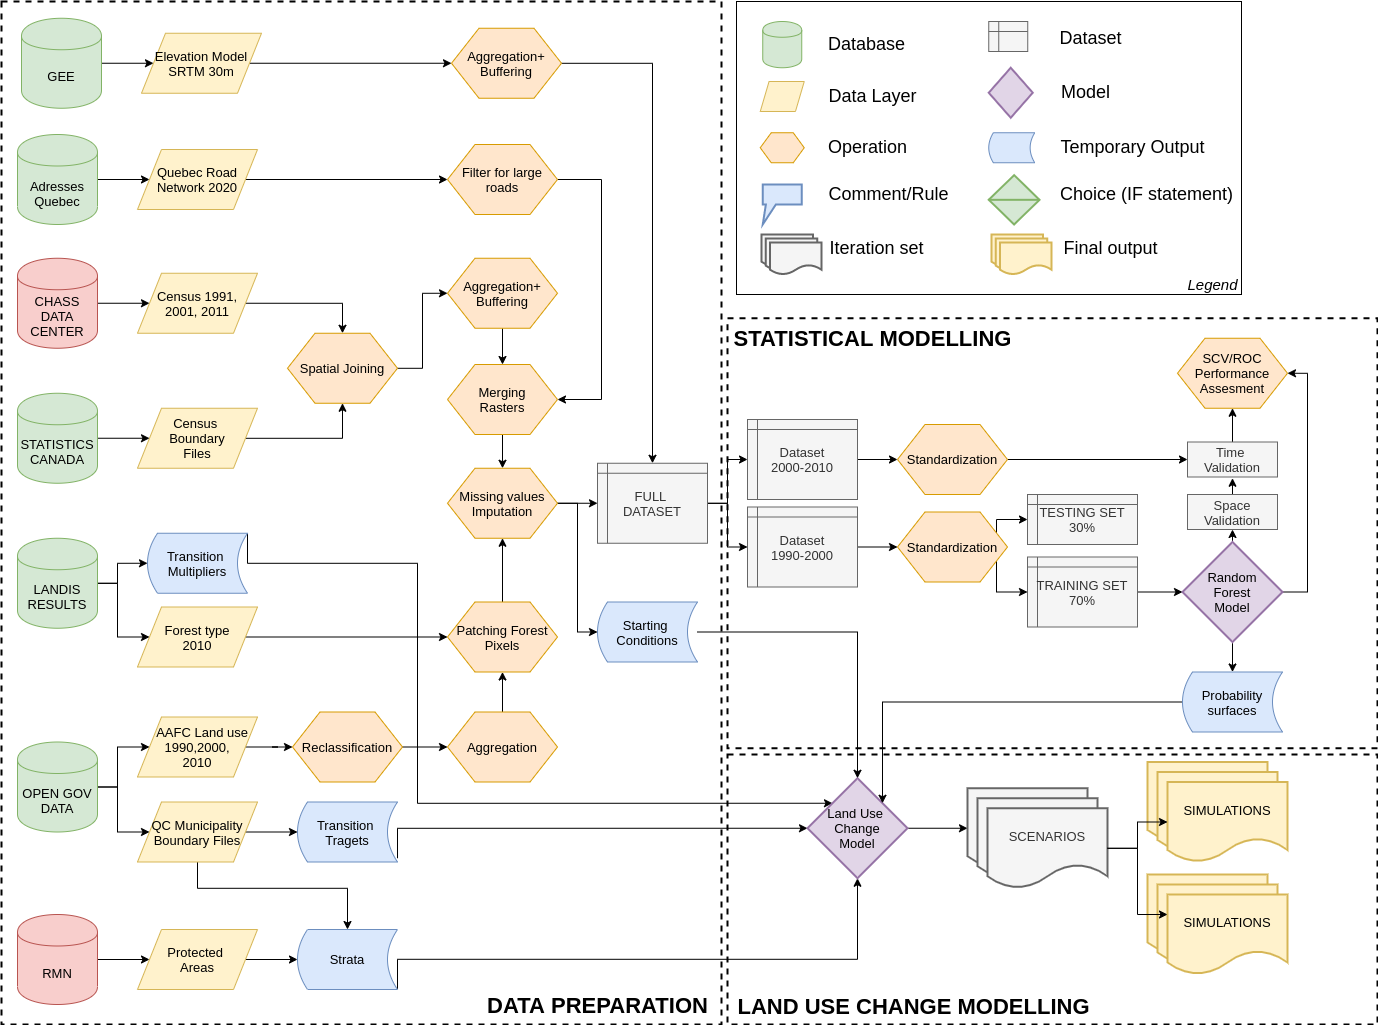
\includegraphics[width=1.3\textwidth]{thesis/figures/Chapter1_flowchart.png}
}
\caption{Workflow for data preparation, statistical modelling and land use change modelling.}
\label{fig:workflow1}
\end{figure}
\clearpage

\begin{figure}[h!]
\makebox[\textwidth]{
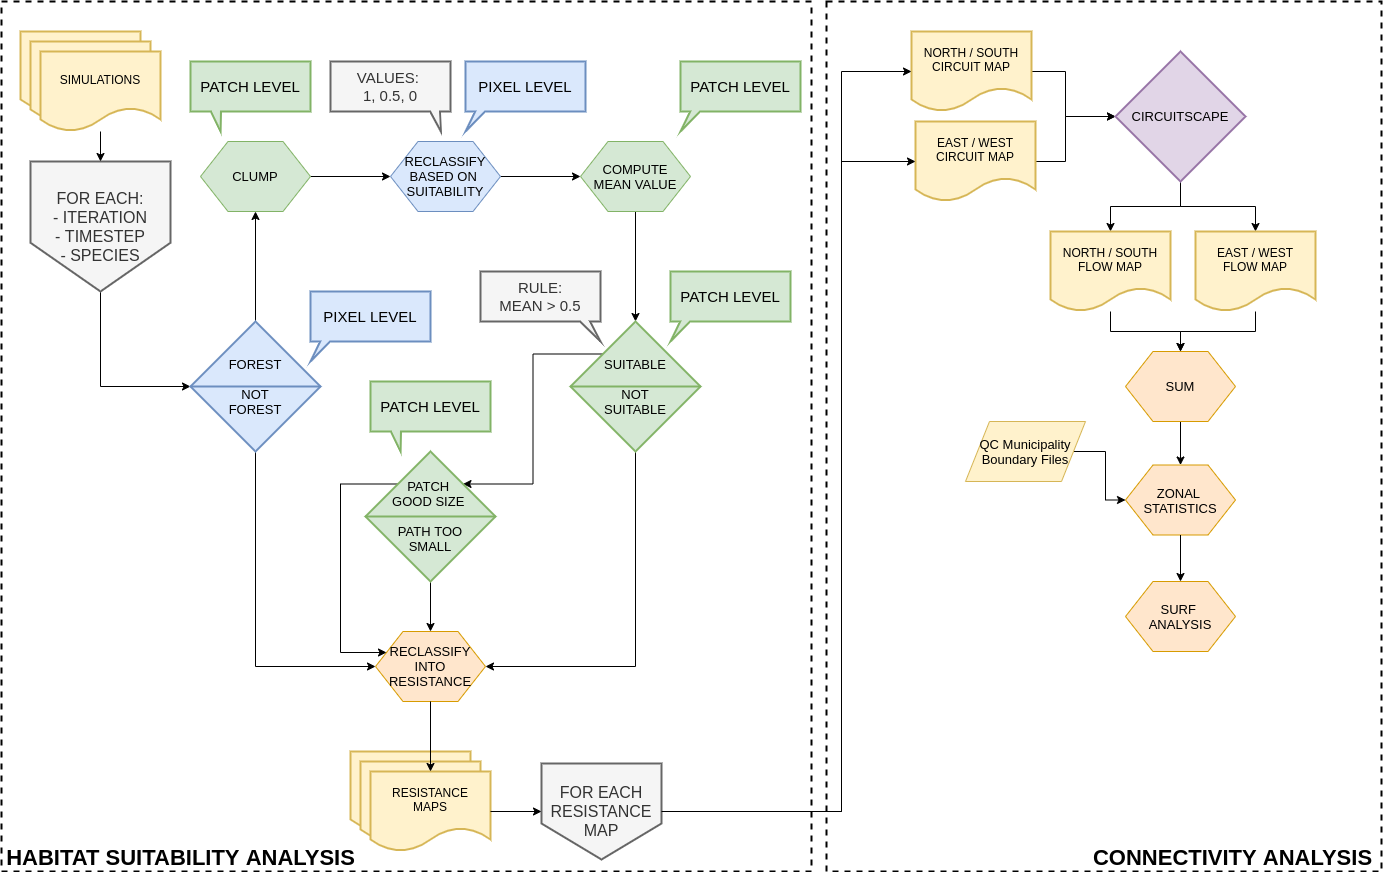
\includegraphics[width=1.3\textwidth]{thesis/figures/Chapter1_flowchart2.png}
}
\caption{Workflow for the habitat suitability and connectivity analyses.} 
\label{fig:workflow2}
\end{figure}
\clearpage

%---------------------------------------------------------------------------------------------------------------------------------------------------
% Results figures

% Figures: values

% Clustering moved to appendix

% PCA
\begin{figure}[h!]
\makebox[\textwidth]{
  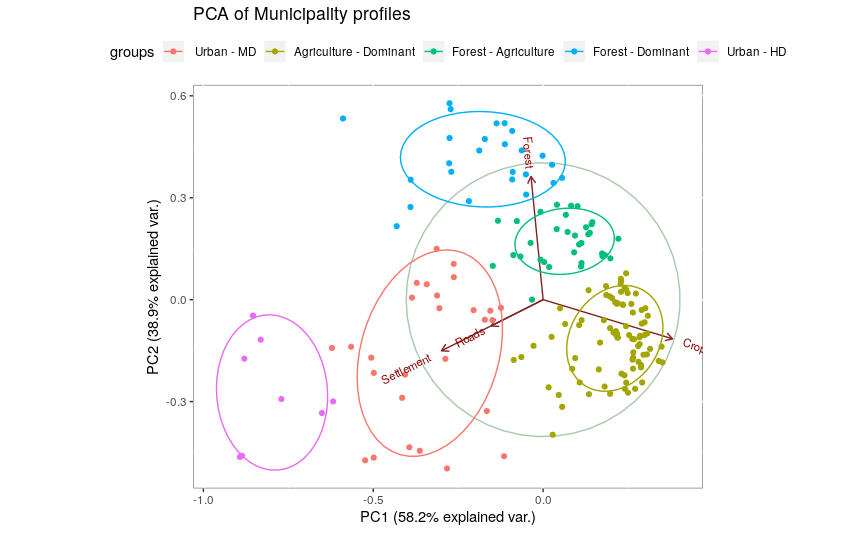
\includegraphics[width=0.9\textwidth]{thesis/figures/PCA_data_profiles.png}
}
\caption{Ordination of land use data (proportions) for municipalities.}
\label{fig:PCAvals}

% MAP
\makebox[\textwidth]{
    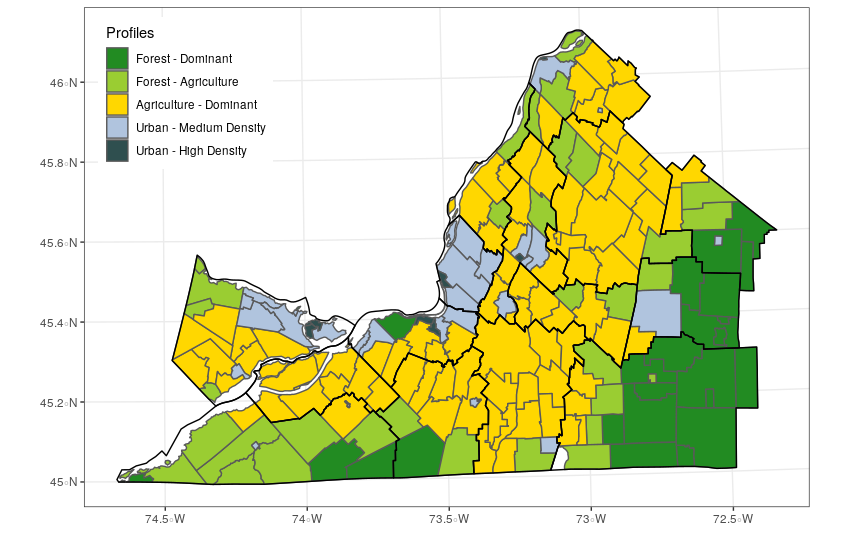
\includegraphics[width=0.9\textwidth]{thesis/figures/profiles_land_use.png}
}
\caption{Geographical distribution of the 5 profiles identified in figure \ref{fig:PCAvals}.}
\label{fig:mapvals}
\end{figure}

% Figures: Transitions

% PCA
\begin{figure}[h!]
\makebox[\textwidth]{
  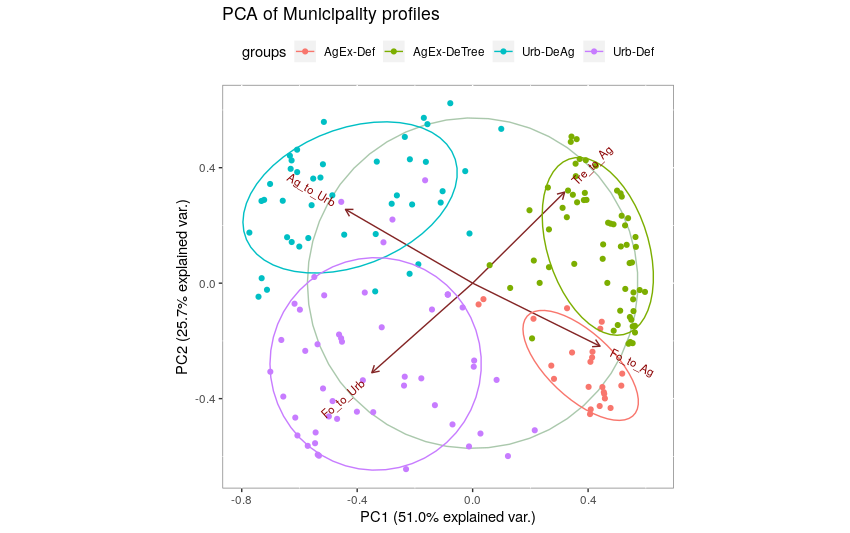
\includegraphics[width=0.9\textwidth]{thesis/figures/PCA_trans_profiles.png}
}
\caption{Ordination of land use transition data for municipalities.}
\label{fig:PCAtrans}

%MAP
\makebox[\textwidth]{
    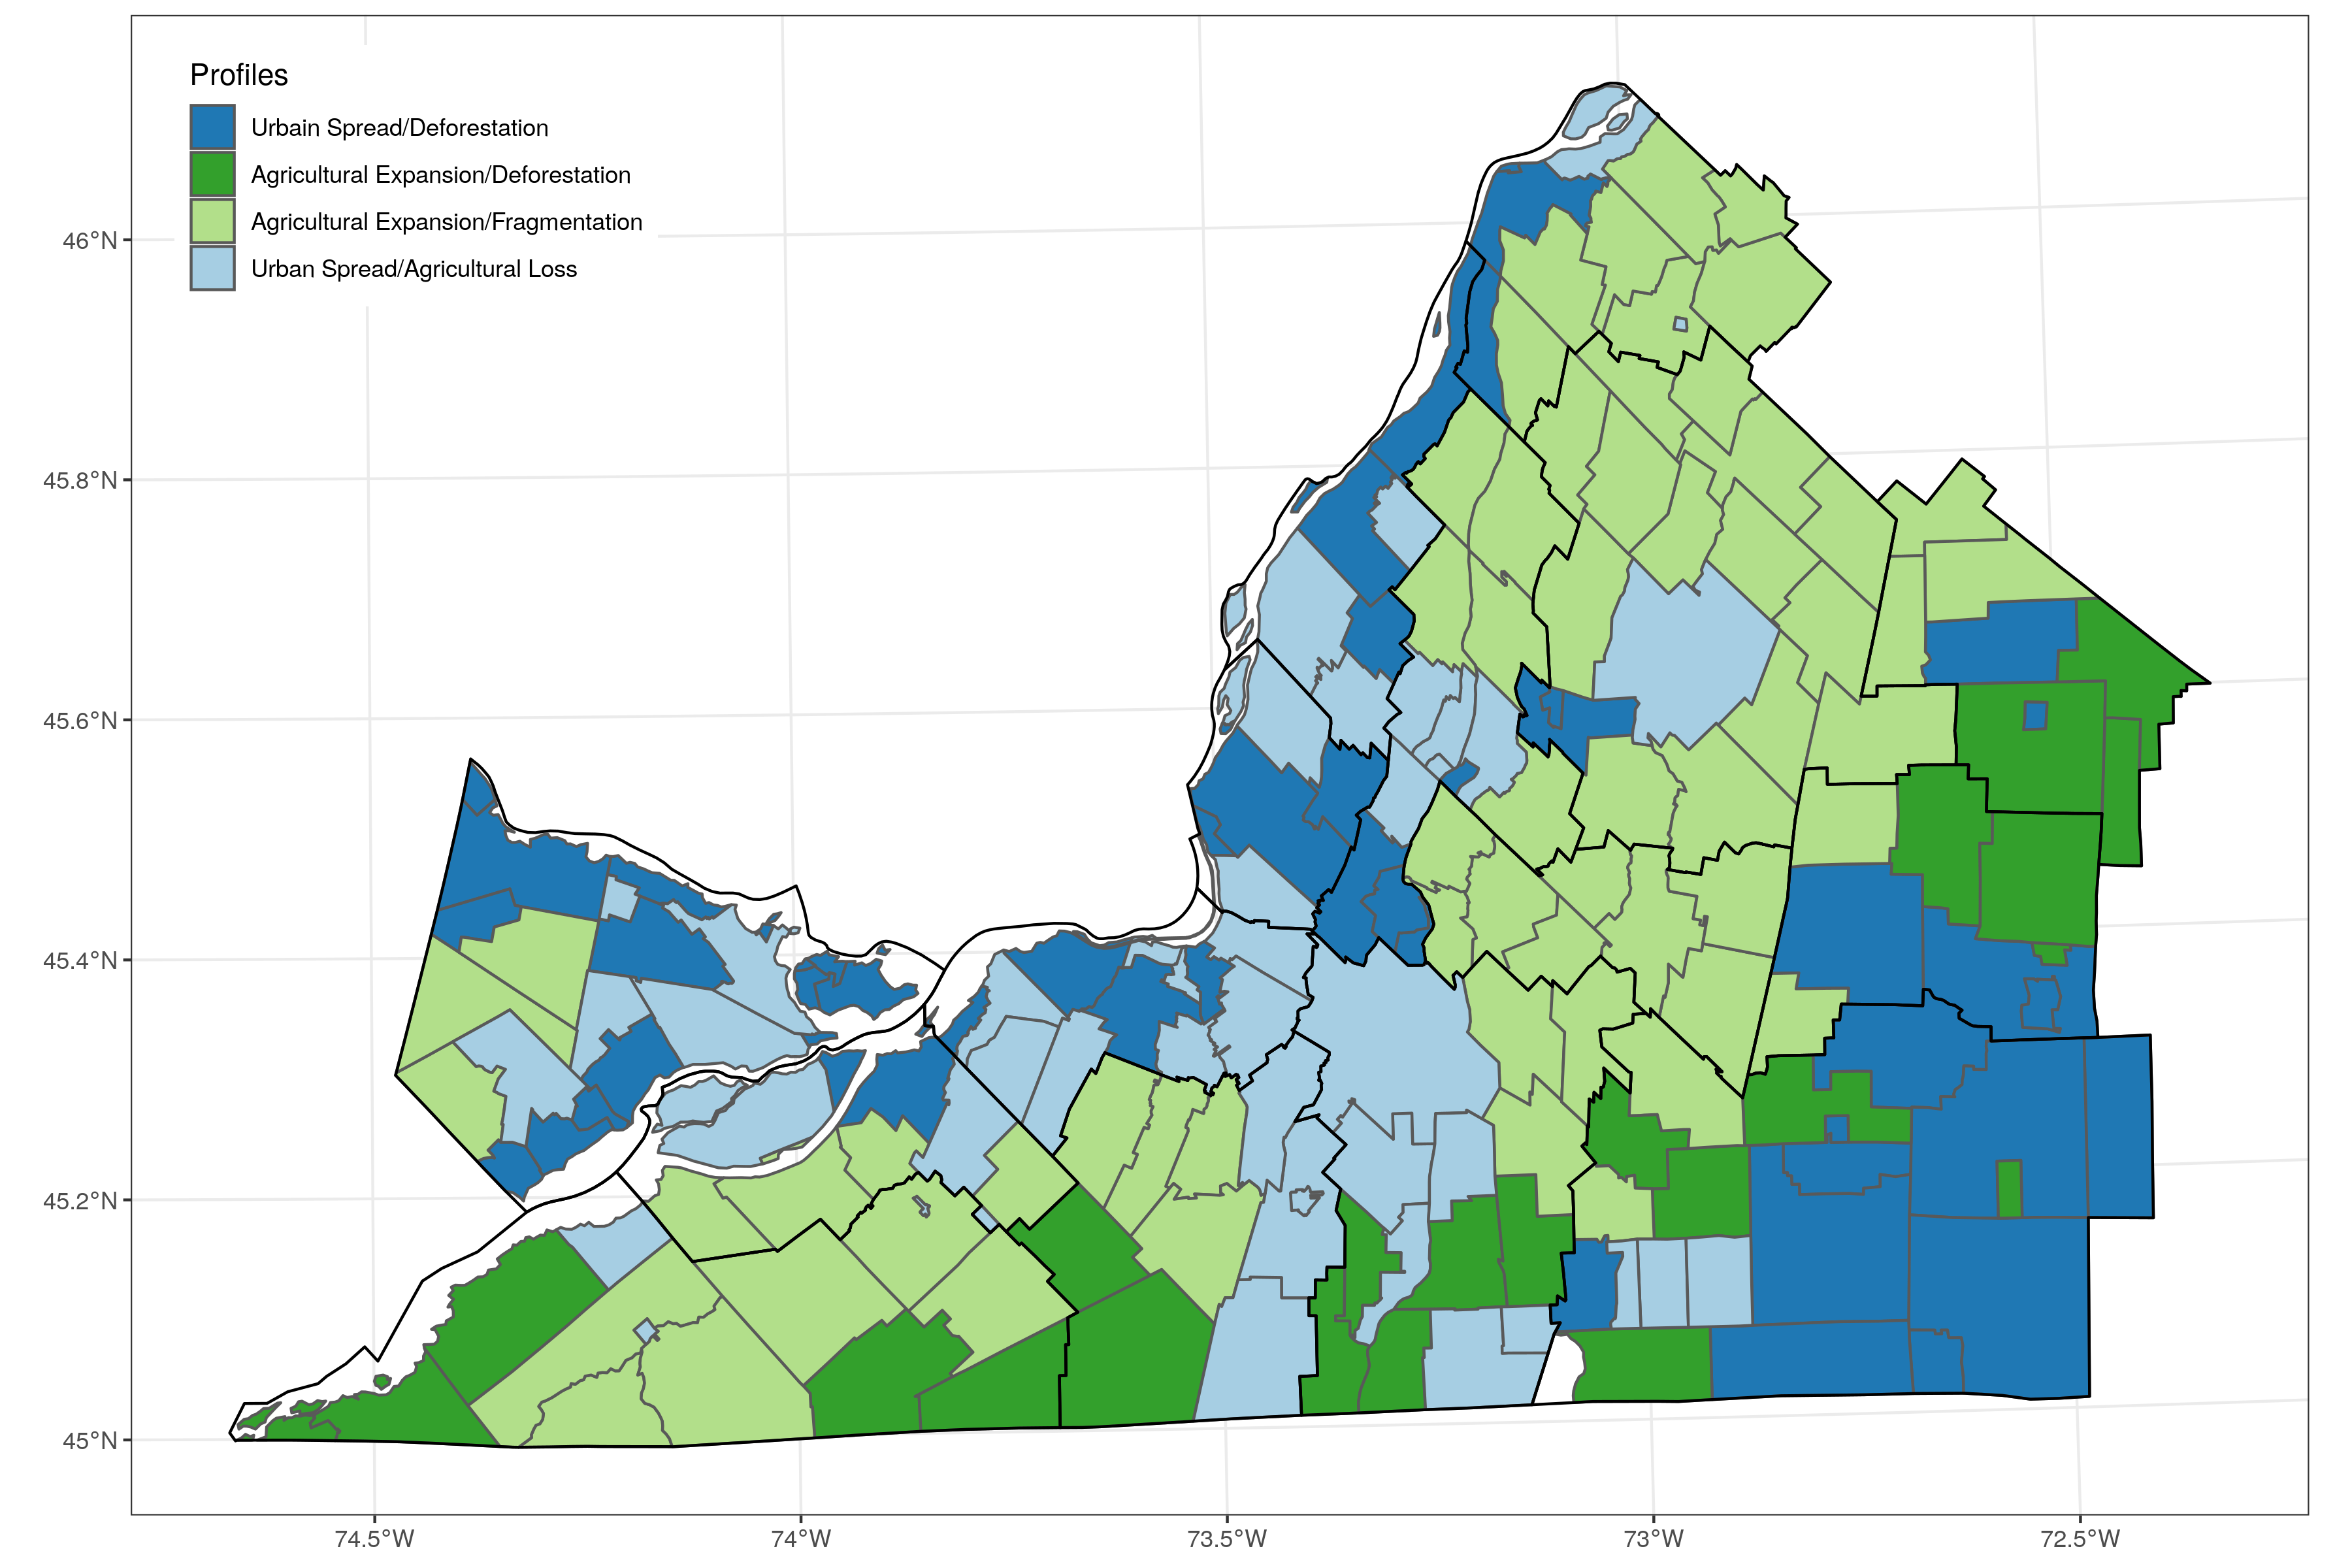
\includegraphics[width=0.9\textwidth]{thesis/figures/transition_prof_map.png}
}
\caption{Geographical distribution of the 4 change profiles identified in figure \ref{fig:PCAtrans}.}
\label{fig:maptrans}
\end{figure}

\clearpage

%---------------------------------------------------------------------------------------------------------------------------------------------------
% Model tables (roc curves moved to the appendix)

% RF Variable importance

\begin{table}[h!]
\centering
\caption{Variable importance (gini impurity index) for both random forest models - non-categorical variables only (rounded to nearest integer, highest values in bold).}
\label{tab:varimp}
\begin{tabular}{lcc}
\hline
\hline
\multicolumn{1}{c}{\multirow{2}{*}{Variable}} & \multicolumn{2}{c}{Model} \\ \cline{2-3} 
\multicolumn{1}{c}{} & \multicolumn{1}{l}{Urbanisation} & \multicolumn{1}{l}{Agricultural expansion} \\ \hline
Distance from urban land & \textbf{2118} & 571 \\
Size of forest patch & 409 & \textbf{8424} \\
Elevation & 184 & 796 \\
Population change & 332 & 297 \\
Income & 371 & 315 \\ 
\hline
\end{tabular}
%\end{table}

% R squares and AUC

%\begin{table}[!htbp] \centering 
  \caption[$R^{2}$, AUC, and average precision values for both models and both validation sets.]{$R^{2}$, AUC, and average precision values for both models and both validation sets - The spatial validation set corresponds to the testing partition for the 1990-2000 timestep, whereas the temporal validation set corresponds to the entire data of the 2000-2010 timestep.} 
  \label{tab:R_squares_AUC} 
\begin{tabular}{@{\extracolsep{5pt}} ccccc} 
\\[-1.8ex]\hline 
\hline \\[-1.8ex] 
Model & Validation set & $R^{2}$ & AUC & Average Precision \\ 
\hline \\[-1.8ex] 
Agricultural Expansion & Spatial & $0.566$ & $0.931$ & $0.652$ \\ 
Agricultural Expansion &  Temporal & $0.566$ & $0.841$ & $0.023$ \\ 
Urbanization & Spatial & $0.573$ & $0.939$ & $0.234$ \\ 
Urbanization & Temporal & $0.573$ & $0.921$ & $0.250$ \\ 
\hline \\[-1.8ex] 
\end{tabular} 
%\end{table} 

% R square resample

%\begin{table}[!htbp] \centering 
\caption{AUC values for both models in resampled 10 folds CCV.} 
\label{tab:R_squares_resample} 
\begin{tabular}{@{\extracolsep{5pt}} cccccc} 
\\[-1.8ex]\hline 
\hline \\[-1.8ex] 
Model & Mean AUC +/- Std \\ 
\hline \\[-1.8ex] 
Agricultural Expansion & $0.929 \pm 0.002$ \\ 
Urbanisation & $0.938 \pm 0.002$ \\ 
\hline \\[-1.8ex] 
\end{tabular}
%\end{table} 

% Historic model metrics

%\begin{table}[!htbp] \centering
\caption{AUC and average precision values for the predictions of the land use change model.} 
\label{tab:historic_metrics} 
\begin{tabular}{lcccc}
\hline
\hline
\multicolumn{1}{c}{Model} & \begin{tabular}[c]{@{}c@{}}Mean AUC\\ (Averaged \\ Surface)\end{tabular} & \begin{tabular}[c]{@{}c@{}}Mean Precision\\ (Averaged \\ Surface)\end{tabular} & \begin{tabular}[c]{@{}c@{}}Mean AUC +/- Std\\ (All Iterations \\ Averaged)\end{tabular} & \begin{tabular}[c]{@{}c@{}}Mean Precision +/- Std\\ (All Iterations \\ Averaged)\end{tabular} \\ \hline
\begin{tabular}[c]{@{}l@{}}Agricultural \\ Expansion\end{tabular} & $0.858$ & $0.383$ & $0.678 \pm 0.002$ & $0.109 \pm 0.002$ \\
Urbanisation & $0.784$ & $0.287$ & $0.647 \pm 0.001$ & $0.135 \pm 0.001$ \\ \hline
\end{tabular}
\end{table}

%---------------------------------------------------------------------------------------------------------------------------------------------------
% Historic model 

\begin{figure}[h!]
\makebox[\textwidth]{
  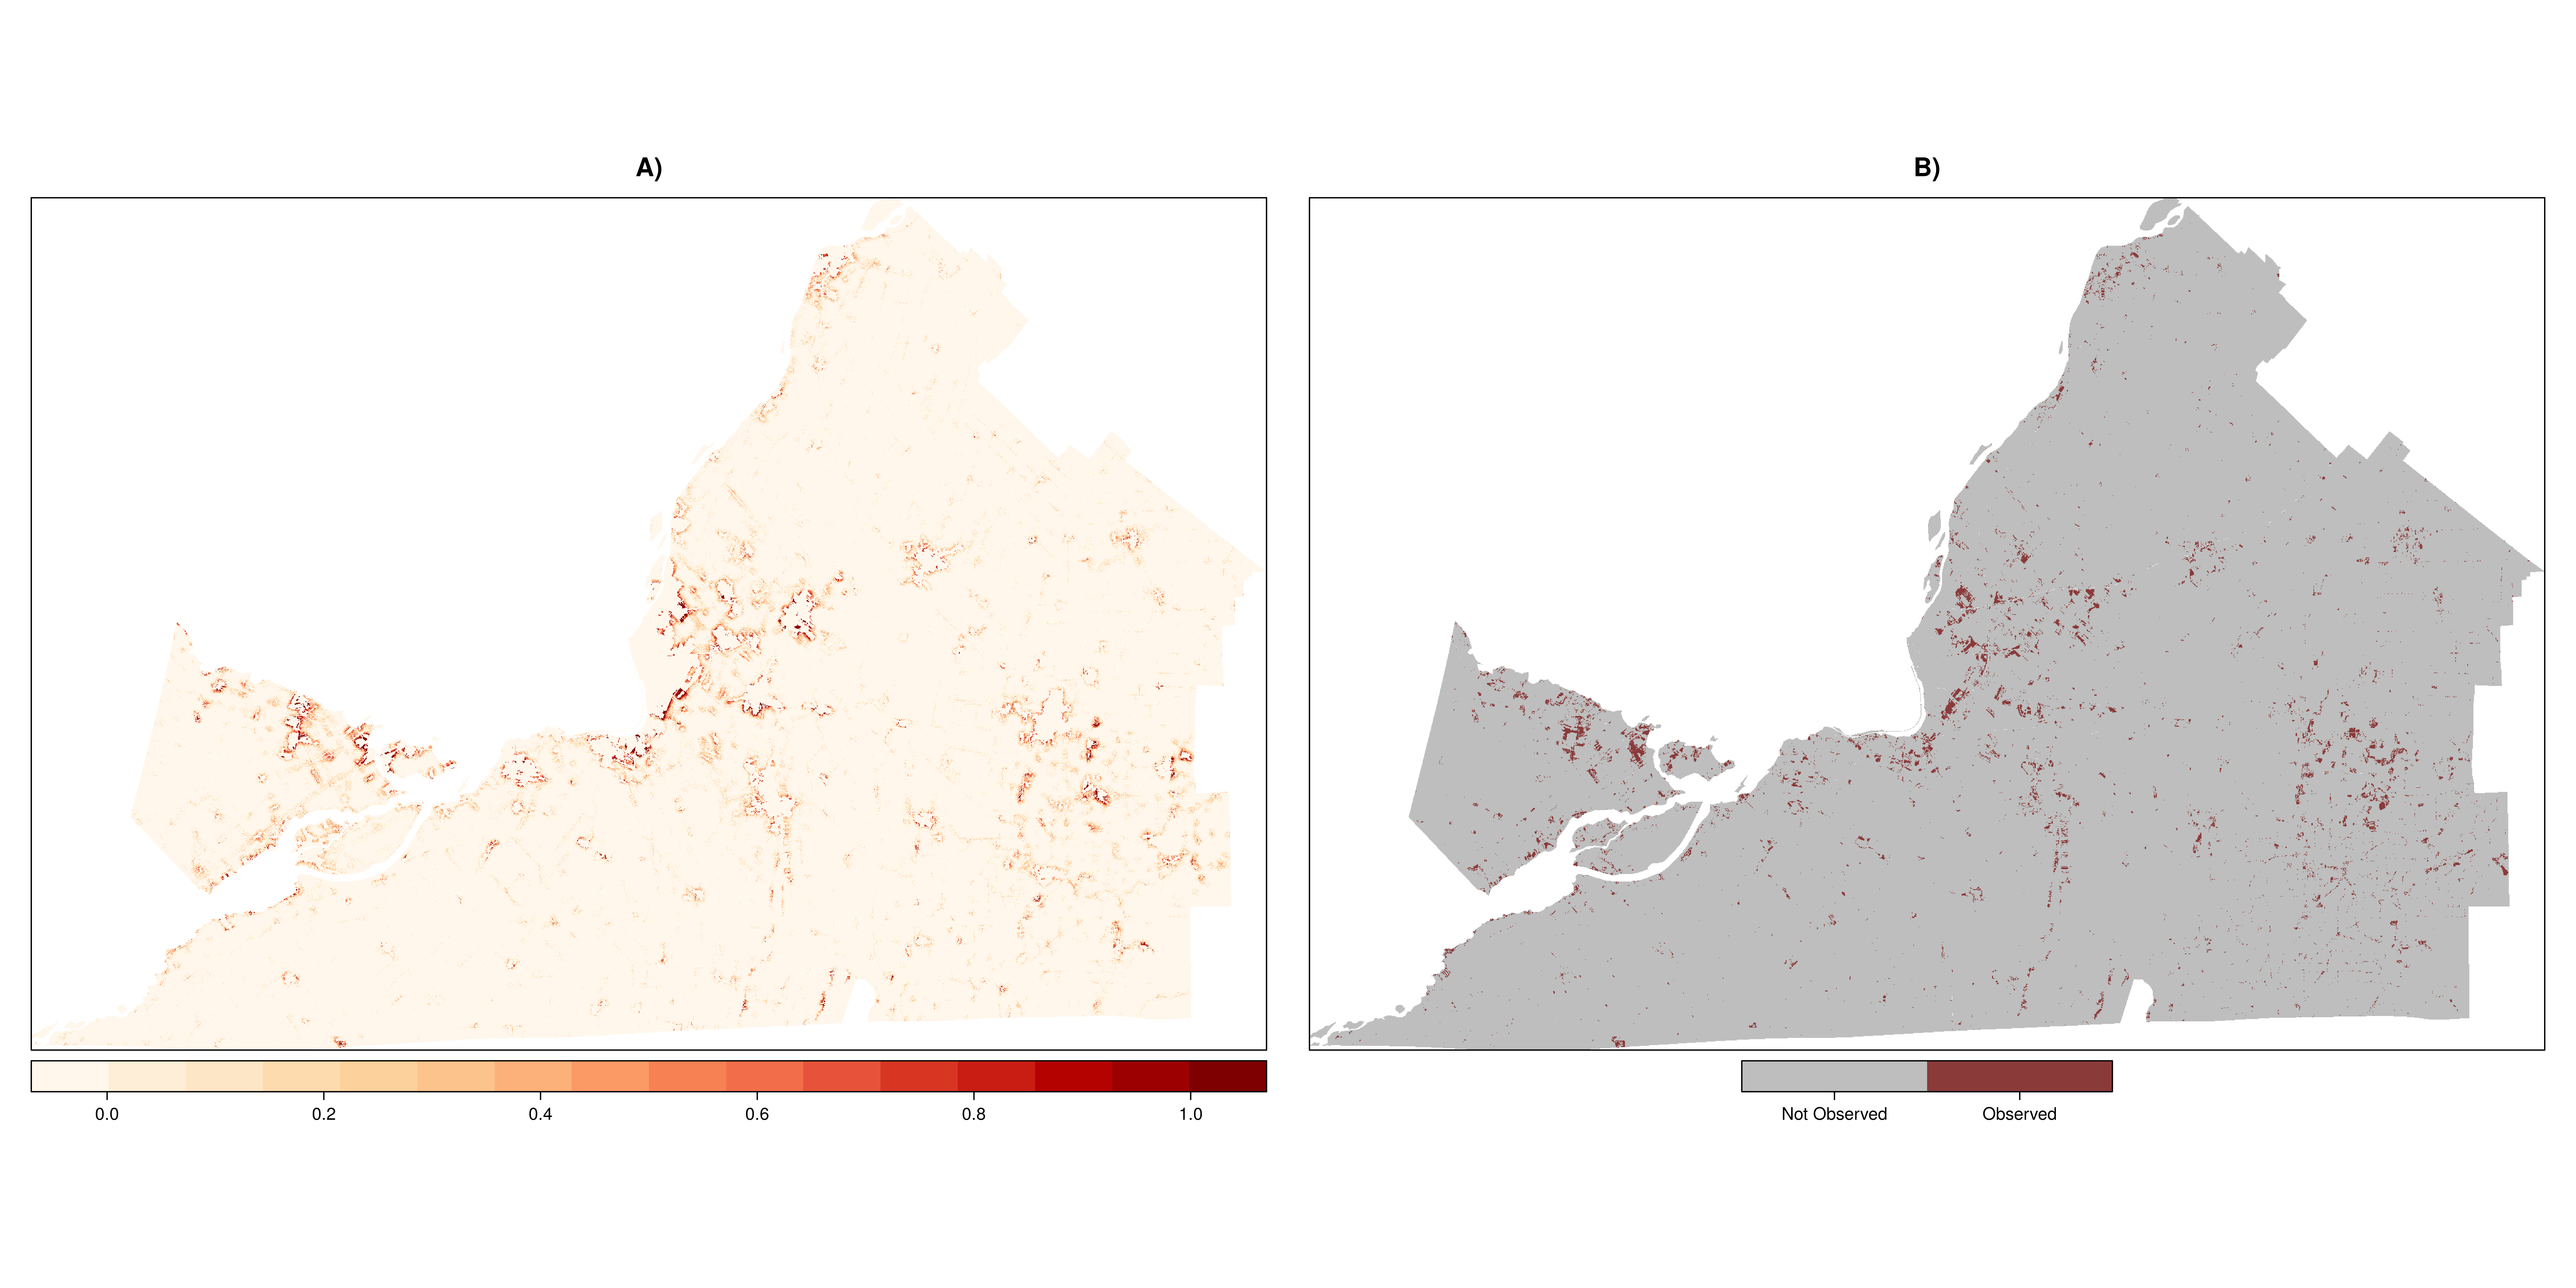
\includegraphics[width=1.3\textwidth]{thesis/figures/historic_compare_urb.png}
}
 \caption[Predicted probability of urbanization vs observed urbanization between 1990 and 2010.]{Predicted probability of urbanization (left) vs observed urbanization (right) between 1990 and 2010.}
 \label{fig:compare_urb}
%\end{figure}

%\begin{figure}[h!]
\makebox[\textwidth]{
  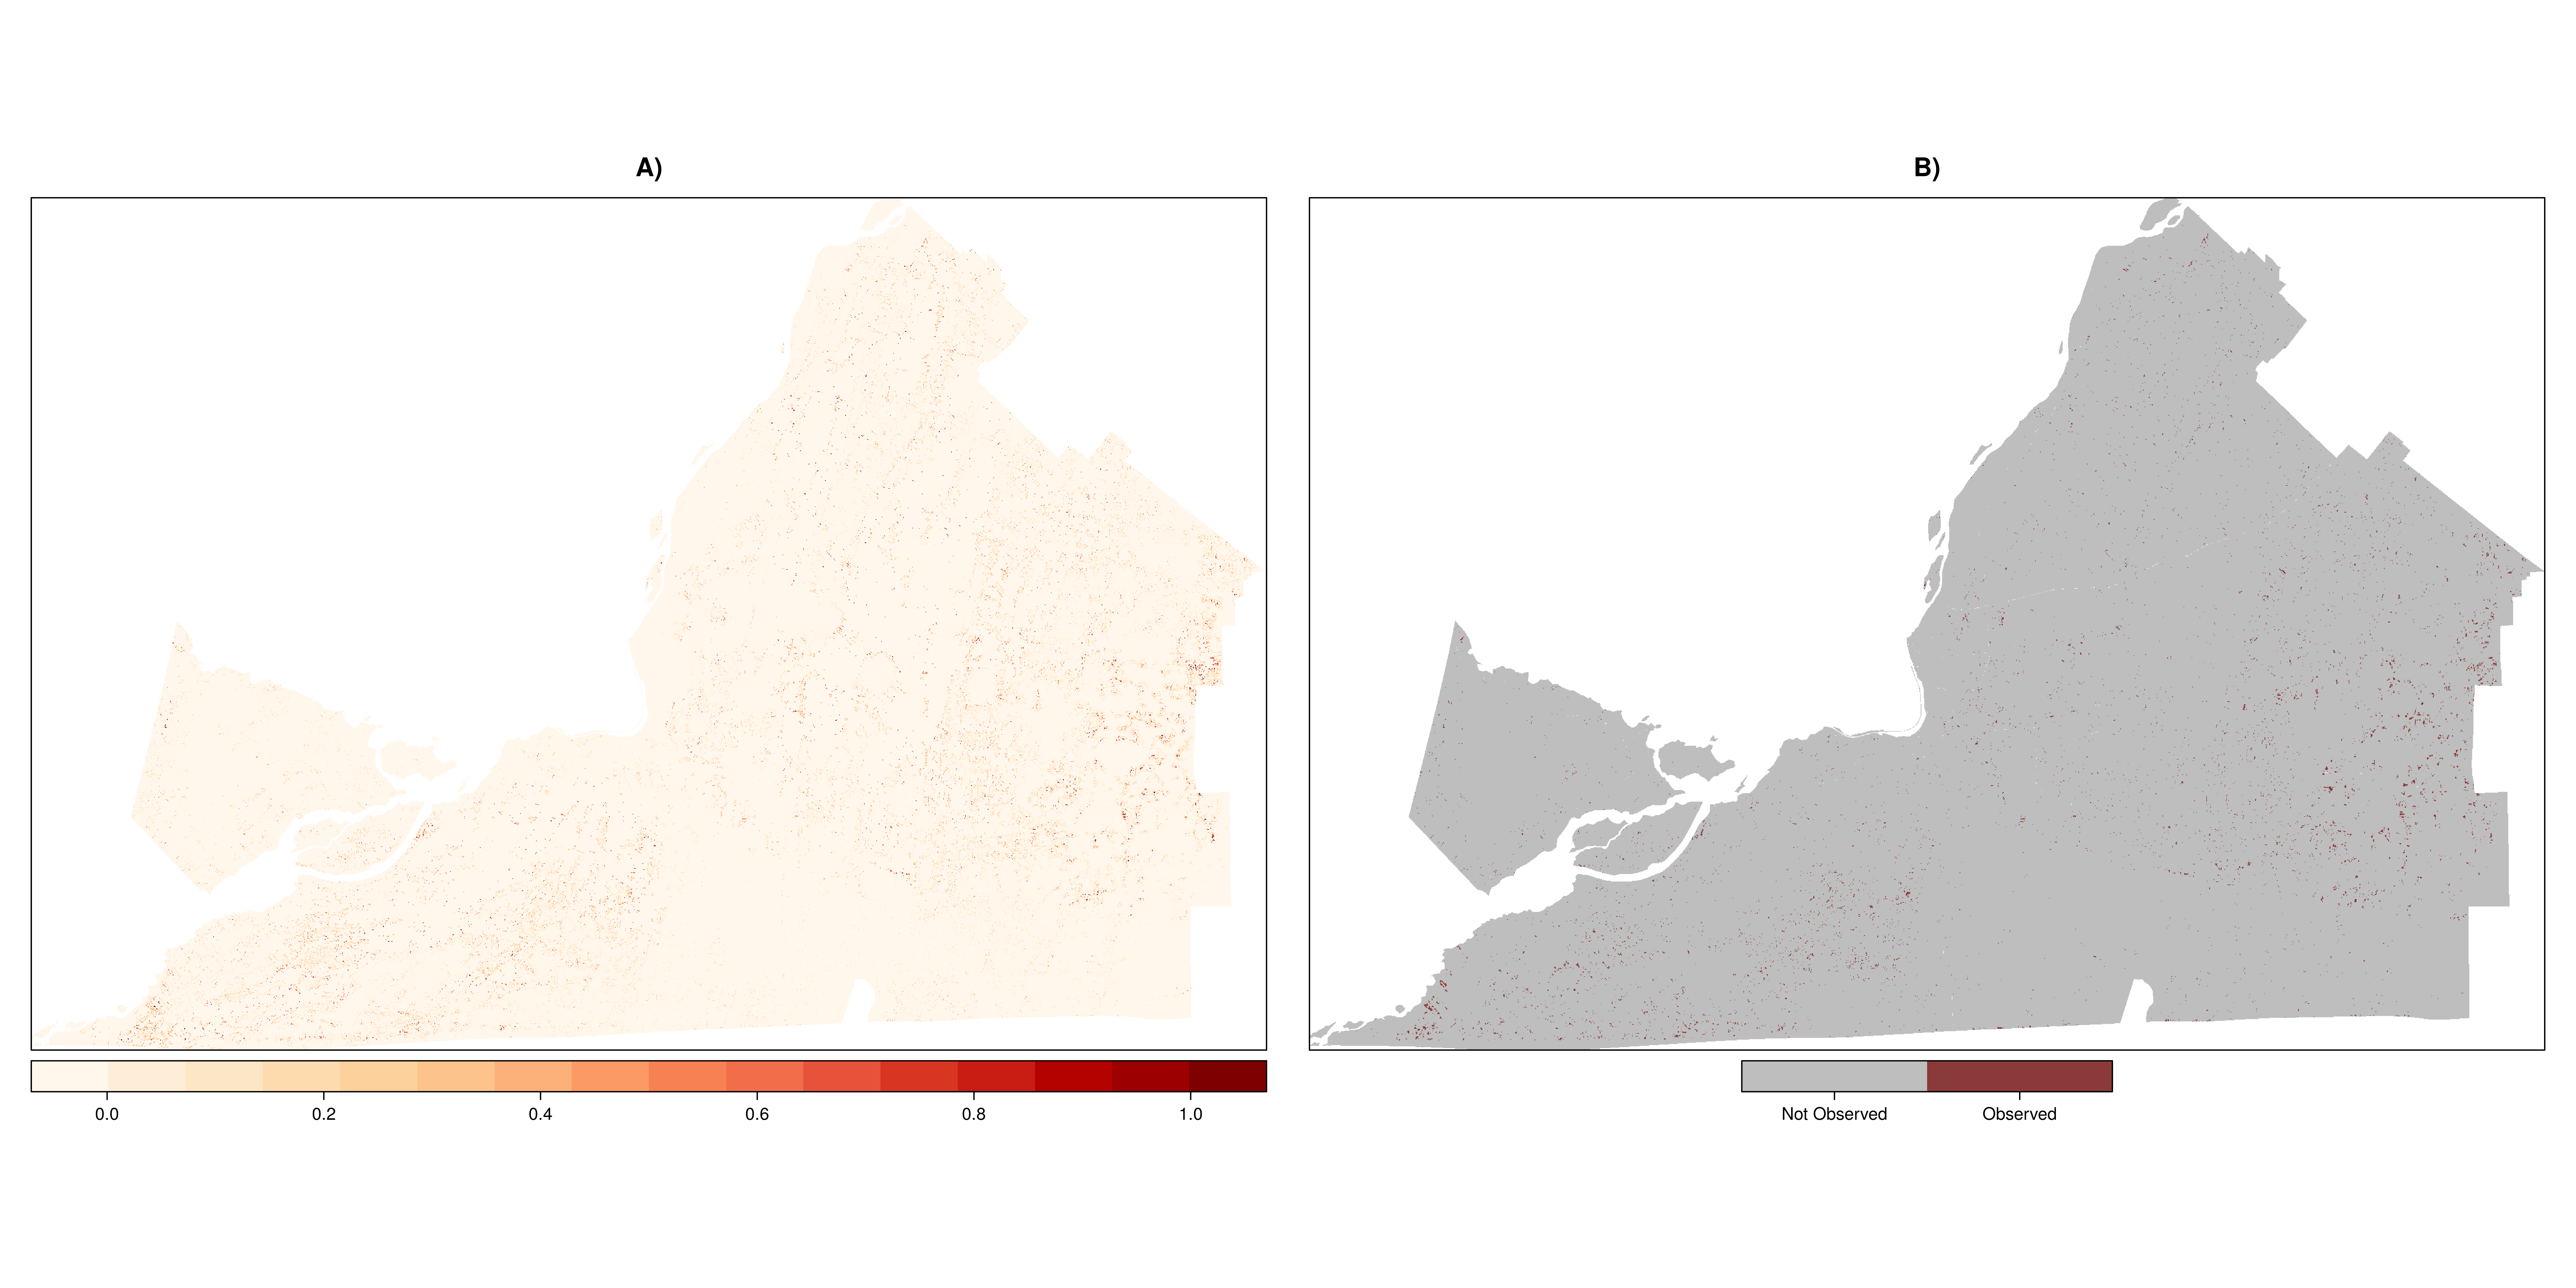
\includegraphics[width=1.3\textwidth]{thesis/figures/historic_compare_agex.png}
}
 \caption[Predicted probability of agricultural expansion vs observed agricultural expansion between 1990 and 2010.]{Predicted probability of agricultural expansion (left) vs observed agricultural expansion (right) between 1990 and 2010.}
 \label{fig:compare_agex}
\end{figure}

%---------------------------------------------------------------------------------------------------------------------------------------------------
% Other land use change scenario (maps moved to appendix)

\begin{figure}[h!]
\makebox[\textwidth]{
  \includegraphics[width=1.3\textwidth]{thesis/figures/bar_both.png}
}
 \caption{Land use class frequencies in 2010 (observed) and 2100 (predicted) for the BAU and Reforestation scenarios (under baseline climate scenario).}
 \label{fig:bar_both}
\end{figure}

%---------------------------------------------------------------------------------------------------------------------------------------------------
% Histogram historic

\begin{figure}[h!]
\makebox[\textwidth]{
  \includegraphics[width=1.3\textwidth]{thesis/figures/original_hists.png}
}
 \caption{Histograms of flow values for the year 2010 comparing the historic model run (1990-2010) with observations.}
 \label{fig:hist_historic}
\end{figure}

%---------------------------------------------------------------------------------------------------------------------------------------------------
% Flow

% Historic

\begin{figure}[h!]
\makebox[\textwidth]{
  \includegraphics[width=1.3\textwidth]{thesis/figures/connectivity_decrease_x5species_historic.png}
}
 \caption{Change in mean flow (in \% of the 1990 flow) between 1990 and 2010, contrasting observed historic change (1990-2010) and simulated change from historic model run.}
 \label{fig:flow_historic}
\end{figure}

% Linear

\begin{figure}[h!]
\makebox[\textwidth]{
  \includegraphics[width=1.3\textwidth]{thesis/figures/connectivity_decrease_x5species_chap1.png}
}
 \caption{Change in mean flow (in \% of the 2010 flow) between 2010 (observed) and 2100 (predicted), contrasting BAU scenario (solid line) with other land use change scenarios - linear graph.}
 \label{fig:flow_linear_1}
\end{figure}

% Radar

\begin{figure}[h!]
\makebox[\textwidth]{
  \includegraphics[width=1.3\textwidth]{thesis/figures/radar_ggradar_chap1.png}
}
 \caption{Change in mean flow (in \% of the 2010 flow) between 2010 (observed) and 2100 (predicted), contrasting BAU scenario with other land use change scenarios - radar graph.}
 \label{fig:flow_radar_1}
\end{figure}

% Histograms

\begin{figure}[h!]
\makebox[\textwidth]{
  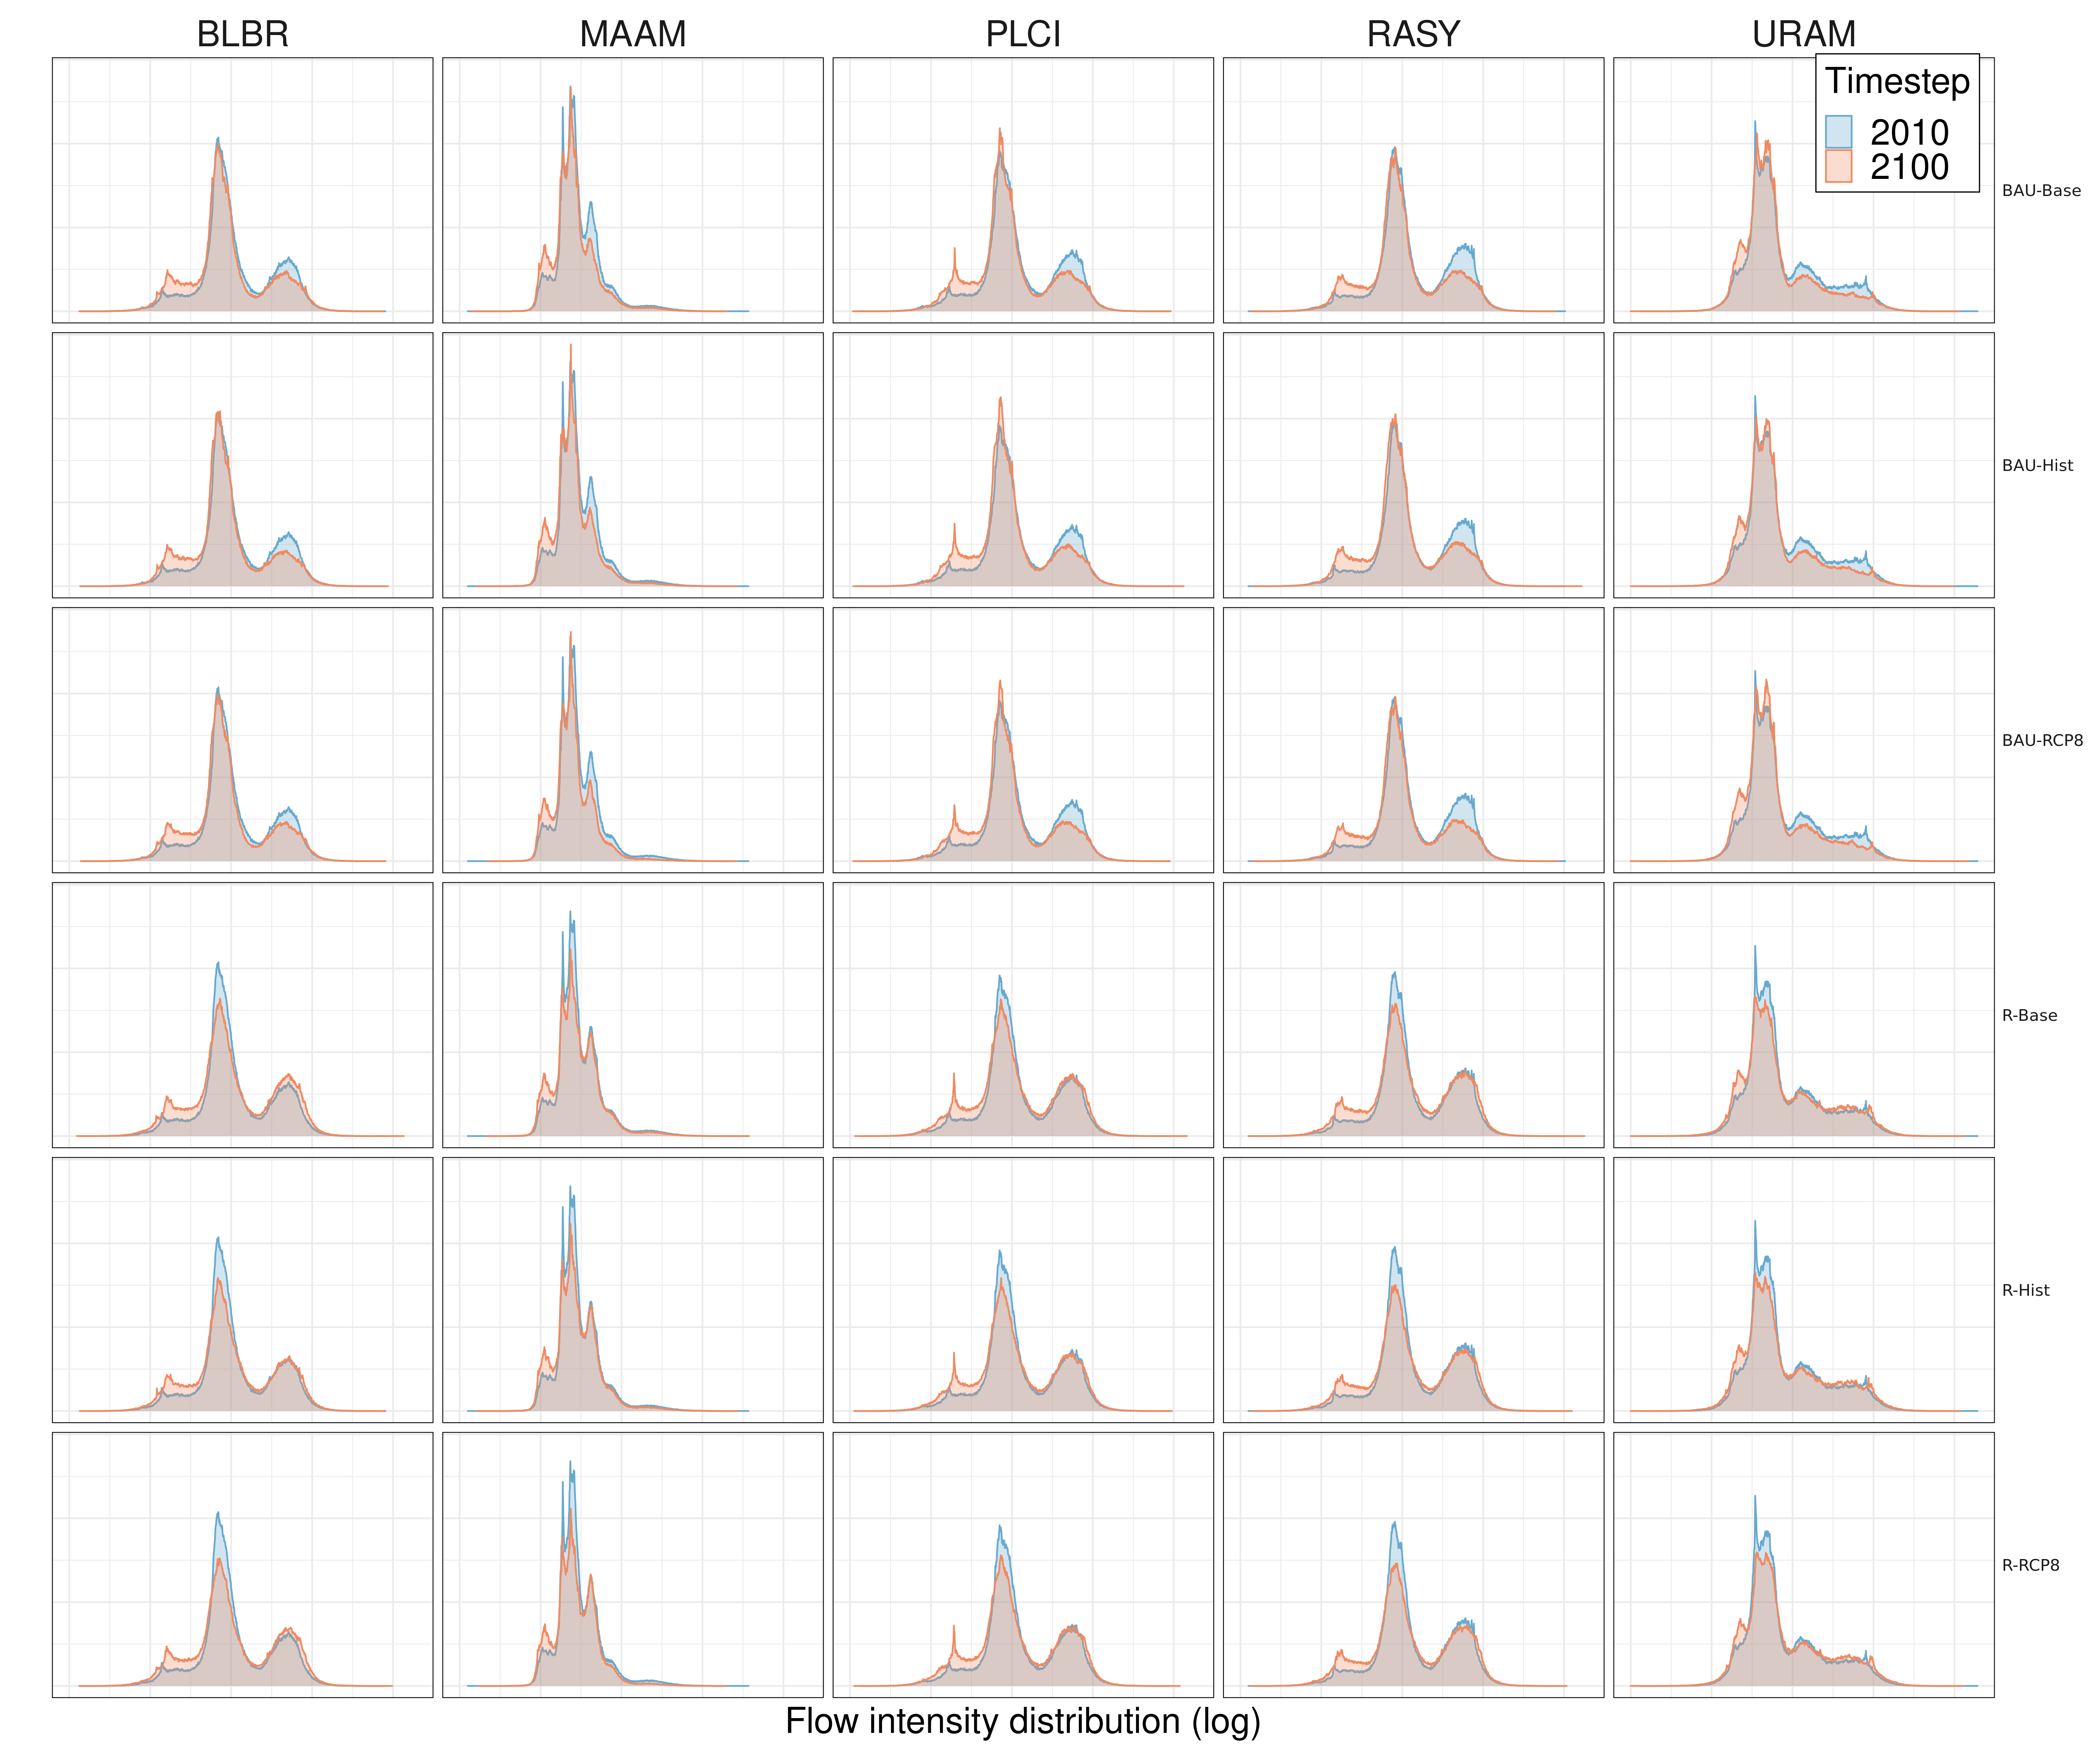
\includegraphics[width=1.3\textwidth]{thesis/figures/hist_chap1.png}
}
 \caption{Histograms of flow values for all species and scenarios, for 2010 (observed) and 2100 (predicted).}
 \label{fig:hist_1}
\end{figure}

%---------------------------------------------------------------------------------------------------------------------------------------------------
% SURF

% Linear

\begin{figure}[h!]
\makebox[\textwidth]{
  \includegraphics[width=1.3\textwidth]{thesis/figures/surf_chap1.png}
}
 \caption{Change in the number of features (in \% of the 2010 flow) identified by the SURF analysis between 2010 (observed) and 2100 (predicted), contrasting BAU scenario with other land use change scenarios - linear graph.}
 \label{fig:surf_linear_1}
\end{figure}

% Radar

\begin{figure}[h!]
\makebox[\textwidth]{
  \includegraphics[width=1.3\textwidth]{thesis/figures/surf_radar_chap1.png}
}
 \caption{Change in the number of features (in \% of the 2010 flow) identified by the SURF analysis between 2010 (observed) and 2100 (predicted), contrasting BAU scenario with other land use change scenarios - radar graph.}
 \label{fig:surf_radar_1}
\end{figure}

%\begin{figure}[h!]
%\makebox[\textwidth]{
%  \includegraphics[width=\textwidth]{figures/.png}
%}
% \caption{}
% \label{fig:}
%\end{figure}

\printbibliography[heading=bibintoc, section=1, title={Chapter 1 Bibliography \hspace{1em}}]

\endrefsection

\newpage
